\chapter{Practical implementation} \label{chap::implementation}
{\it \centering In this chapter, implementation aspects of impact-based SLAM using Sphero robots is presented. Section~\ref{sec::sphero} discusses sensing modalities and characteristics of Sphero robotic ball specific to impact-based SLAM. The practical results of SLAM using a single robot are provided in Section~\ref{sec::single_slam}, followed by map-merging using multiple robots in Section~\ref{sec::map_merge}.}

\section{Sphero robot} \label{sec::sphero}
Sphero is a robotic ball developed by Orobotix Inc.\ and is essentially a segway robot enclosed in a hollow spherical shell (See Figure~\ref{sphero_ball}). As the segway moves using its rubber tires, the friction between the shell and tires make the robot move. The unicycle-like robot can spin around the same position and can roll in any commanded direction. 

\begin{figure}
\centering

\includegraphics[scale=0.25]{./images/sphero_revealed}
\caption[Sphero 2.0 Robotic ball]{Sphero 2.0 Robotic ball}
\label{sphero_ball}
\end{figure}

Sphero has been released into the commercial market as a toy robot which can be controlled using a smart phone and an unofficial \acf{SDK} such as ROS \cite{spheroros} is available for doing project work. A detailed background and technical specifications of the robotic ball can be found in \cite{spherorobot}.

Sphero is equipped with an onboard Inertial Measurement Unit (IMU) comprising of 3-axis accelerometer and 3-axis gyroscope. This sensor, called a proprioceptive sensor, provides the sole sensing information for solving impact-based SLAM. As said before, achieving SLAM using minimal sensing information is one of the motivations for this thesis. 

To solve SLAM, information about the robot's pose as well as from the landmarks in a given environment is necessary. The pose information from the robot is acquired from IMU through dead-reckoning. However, this information is subject to drift due to various error sources such as 
\begin{itemize}
\item Limited resolution during integration (time increments, measurement resolution)
\item Internal wheel slip with shell
\end{itemize}

These error sources have to be filtered out using a filter provided the error accumulated in the state estimates are independent of each other. 

The information from the landmarks in a given environment is obtained using the same IMU sensor. Landmarks are observed through collision detection where Sphero collides with the walls of the environment randomly. Example~\ref{ex_head} shows the collision detection technique used for impact-based SLAM.

\begin{exmp}
The collision detection in Sphero is obtained by monitoring the changes in accelerometer data. Figures~\ref{ball_scoll}~and~\ref{ball_scoll2} show accelerometer-time plots from Sphero when a collision detection occurs. At the instant of collision, the accelerometer data dips due to deceleration since the robot comes to rest momentarily. The impact force applied by the robot on the wall is given by the equation,
\begin{equation*}
F = m\cdot a
\end{equation*}
where $m$ is mass of the robot and $a$ is the acceleration. 

\begin{figure}
\centering
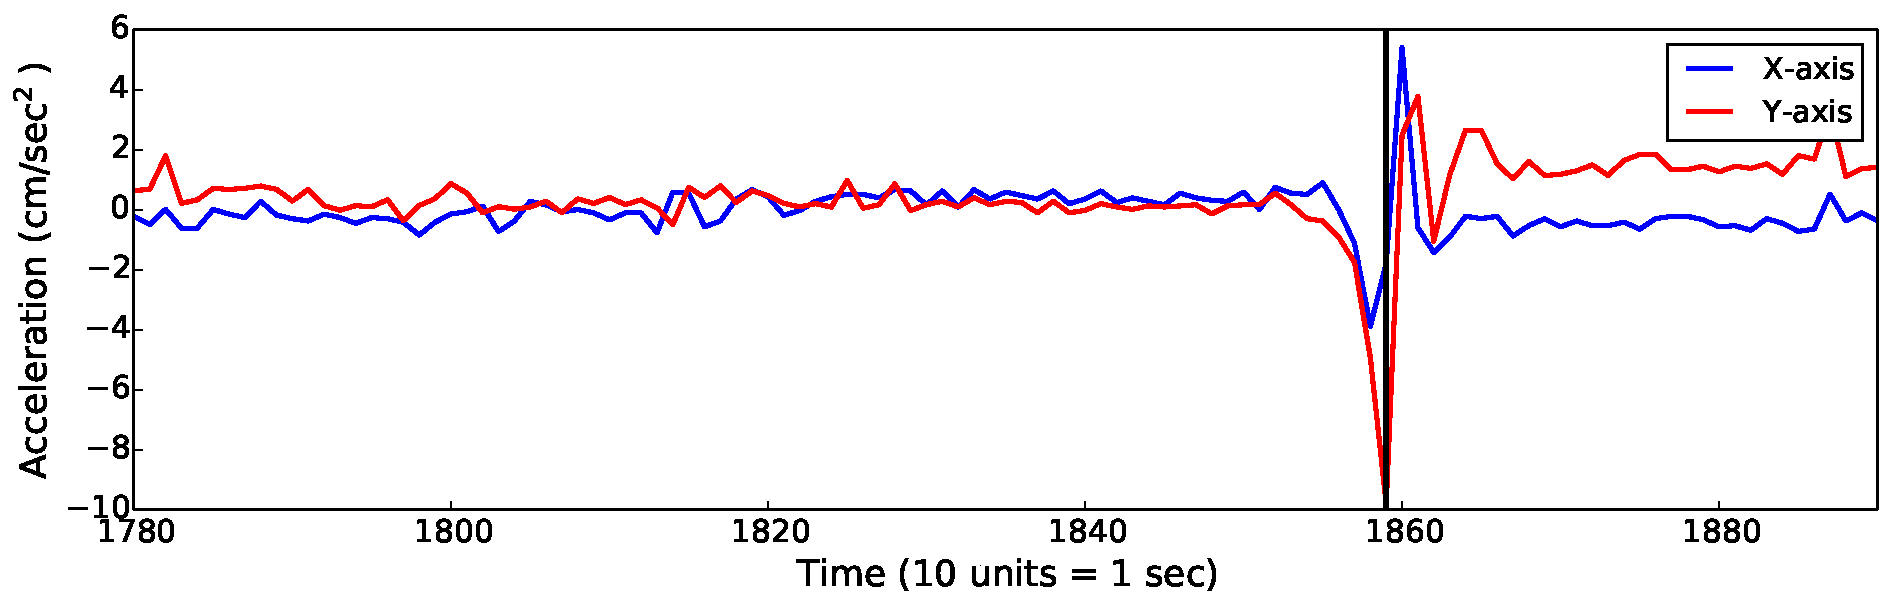
\includegraphics[scale=0.4]{./images/acc_data}
\caption{Effect of impact on X and Y axis accelerometer data. The ball in this case is forced to be at rest. The collision is detected at the black vertical line.}
\label{ball_scoll}
\end{figure}
\begin{figure}
\centering
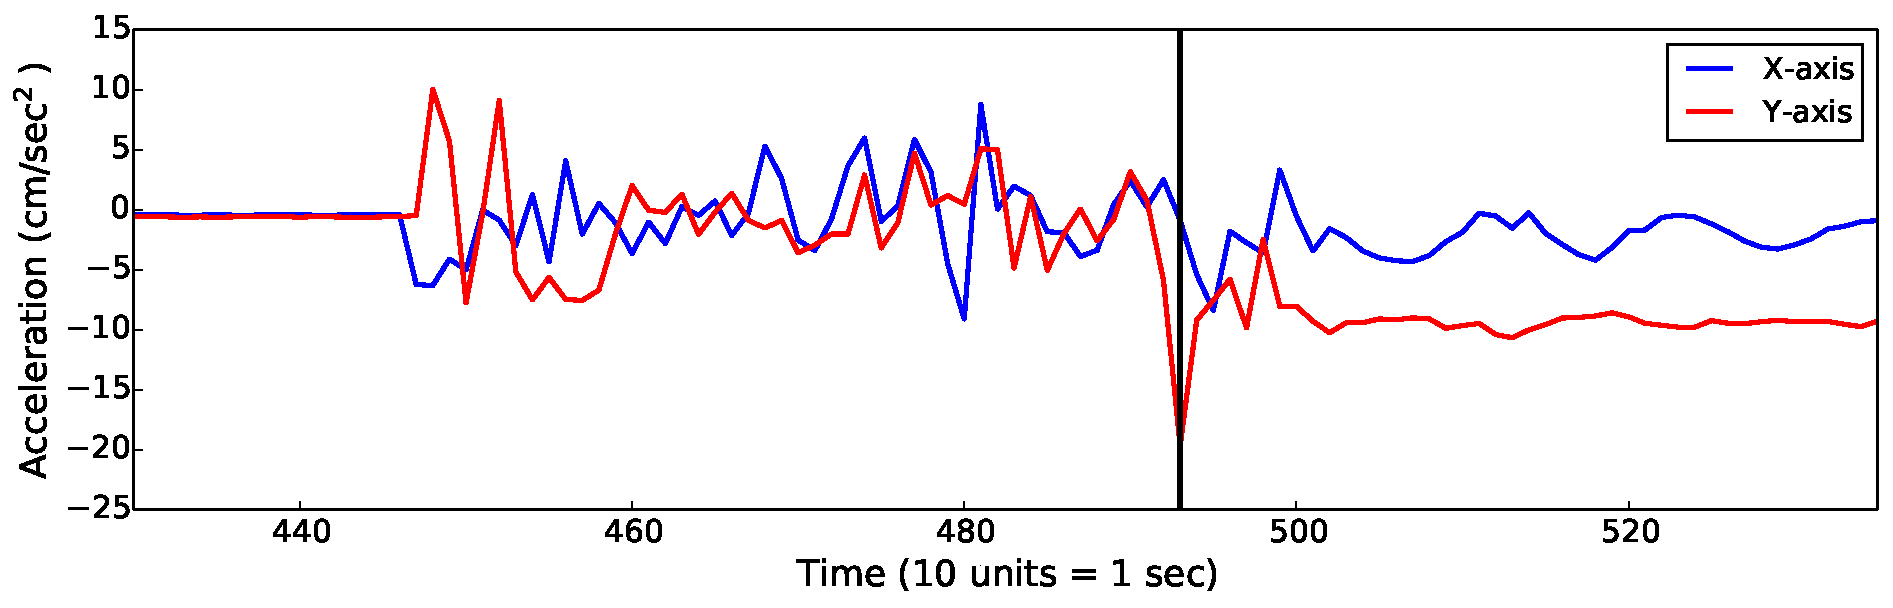
\includegraphics[scale=0.4]{./images/acc_data2}
\caption{Effect of collision on X and Y axis accelerometer data. The ball with a non-zero initial velocity collides against a wall. The collision is detected at the black vertical line.}
\label{ball_scoll2}
\end{figure}

The reaction force experienced by the robot from the wall is ideally same as the impact force and the rate of change of this reaction force (equal to `jerk') is used for computing the wall orientation. 

As the mass $m$ is a constant, wall orientation can also be computed equivalently from the rate of change in acceleration along the X axis and Y axis. For this example, the rate of change in acceleration is computed from the accelerometer plot (Figure~\ref{ball_scoll2}) and the ratio is used to infer the new heading (refer Equation~\ref{t2_orientation}).

The initial robot orientation for the moving robot example in Figure~\ref{ball_scoll2} is 0 radians. The new heading is found from the left/right handed collision model and is close to $\pi$ radians for $c=0$.
\label{ex_head}
\end{exmp}

\section{Single robot SLAM}	\label{sec::single_slam}
The particle filter-SLAM algorithm, developed in Chapter~\ref{chap::solution}, uses the robot's odometry and collision measurements. The pseudo-code for the impact-based SLAM algorithm is provided in Appendix~\ref{chap::pseudocode}. The real world test was carried out with a particle size $M=30$ and an increased accuracy is observed from $M =5$ to $M=25$. The experiment and computations were carried out on a 1.6GHz Xeon workstation and the measurements are provided at a frequency of 16Hz.

The control action applied to the robot is in a random fashion with the next action only depending upon the inference from the current wall collision. The control inputs or actions are robot speed and heading angle, out of which the former is not controlled and is set to a constant value depending upon the operating conditions such as size of the environment. The latter one, heading angle of the robot, must be modified after every collision and as said, the angle is chosen randomly from a given set or it can be assigned using Equations~\ref{t1_orientation}~and~\ref{t2_orientation} with a pre-determined value of constant $c$. 

From the motion models described through a FSM (Figure~\ref{fsm4}), the constant $c$ has to be defined for impact-based collisions. A simple strategy is to go for a reflective collision (angle of incidence is same as angle of reflection) in ball movements ($c=2$) which was followed in the simulations. This approach was found to be very poor in practical scenarios due to huge orientation error accumulating after every collision. The main reason for this orientation error is the slip between the segway-like robot and the hollow shell. The robot heading is found to differ from the actual orientation (yaw axis) by atleast $2\pi$ for 3 to 5 consecutive collisions. Calibration of this error is difficult to be performed online since it involves destabilizing the robot which is time consuming and prone to position errors\footnote{Destabilization involves making the robot stationary and during this phase, the robot exhibits an unusual motion that gets accumulated into the odometry.}. Hence, the robot heading is restricted to a set of values which has the inner slip-less (ideally) collision and this approach is found to have a lower orientation error, suitable for practice. The set of possible headings is unit normal directions of wall hyperplanes where the initial orientation is computed from the first collision. However with head-on collisions, the robot has a higher orientation error from drift in IMU when the robot turns around by $\pi$ radians.        

With random control inputs from the set, impact-based SLAM is implemented for an indoor environment of dimensions $280\text{cm} \times 280\text{cm}$ as shown in Figure~\ref{maze}. The maximum likelihood solution is obtained by choosing particle with highest importance weight in the particle set. The resulting output map of SLAM solution is shown in Figure~\ref{single_lcmap}.

\begin{figure}
\centering
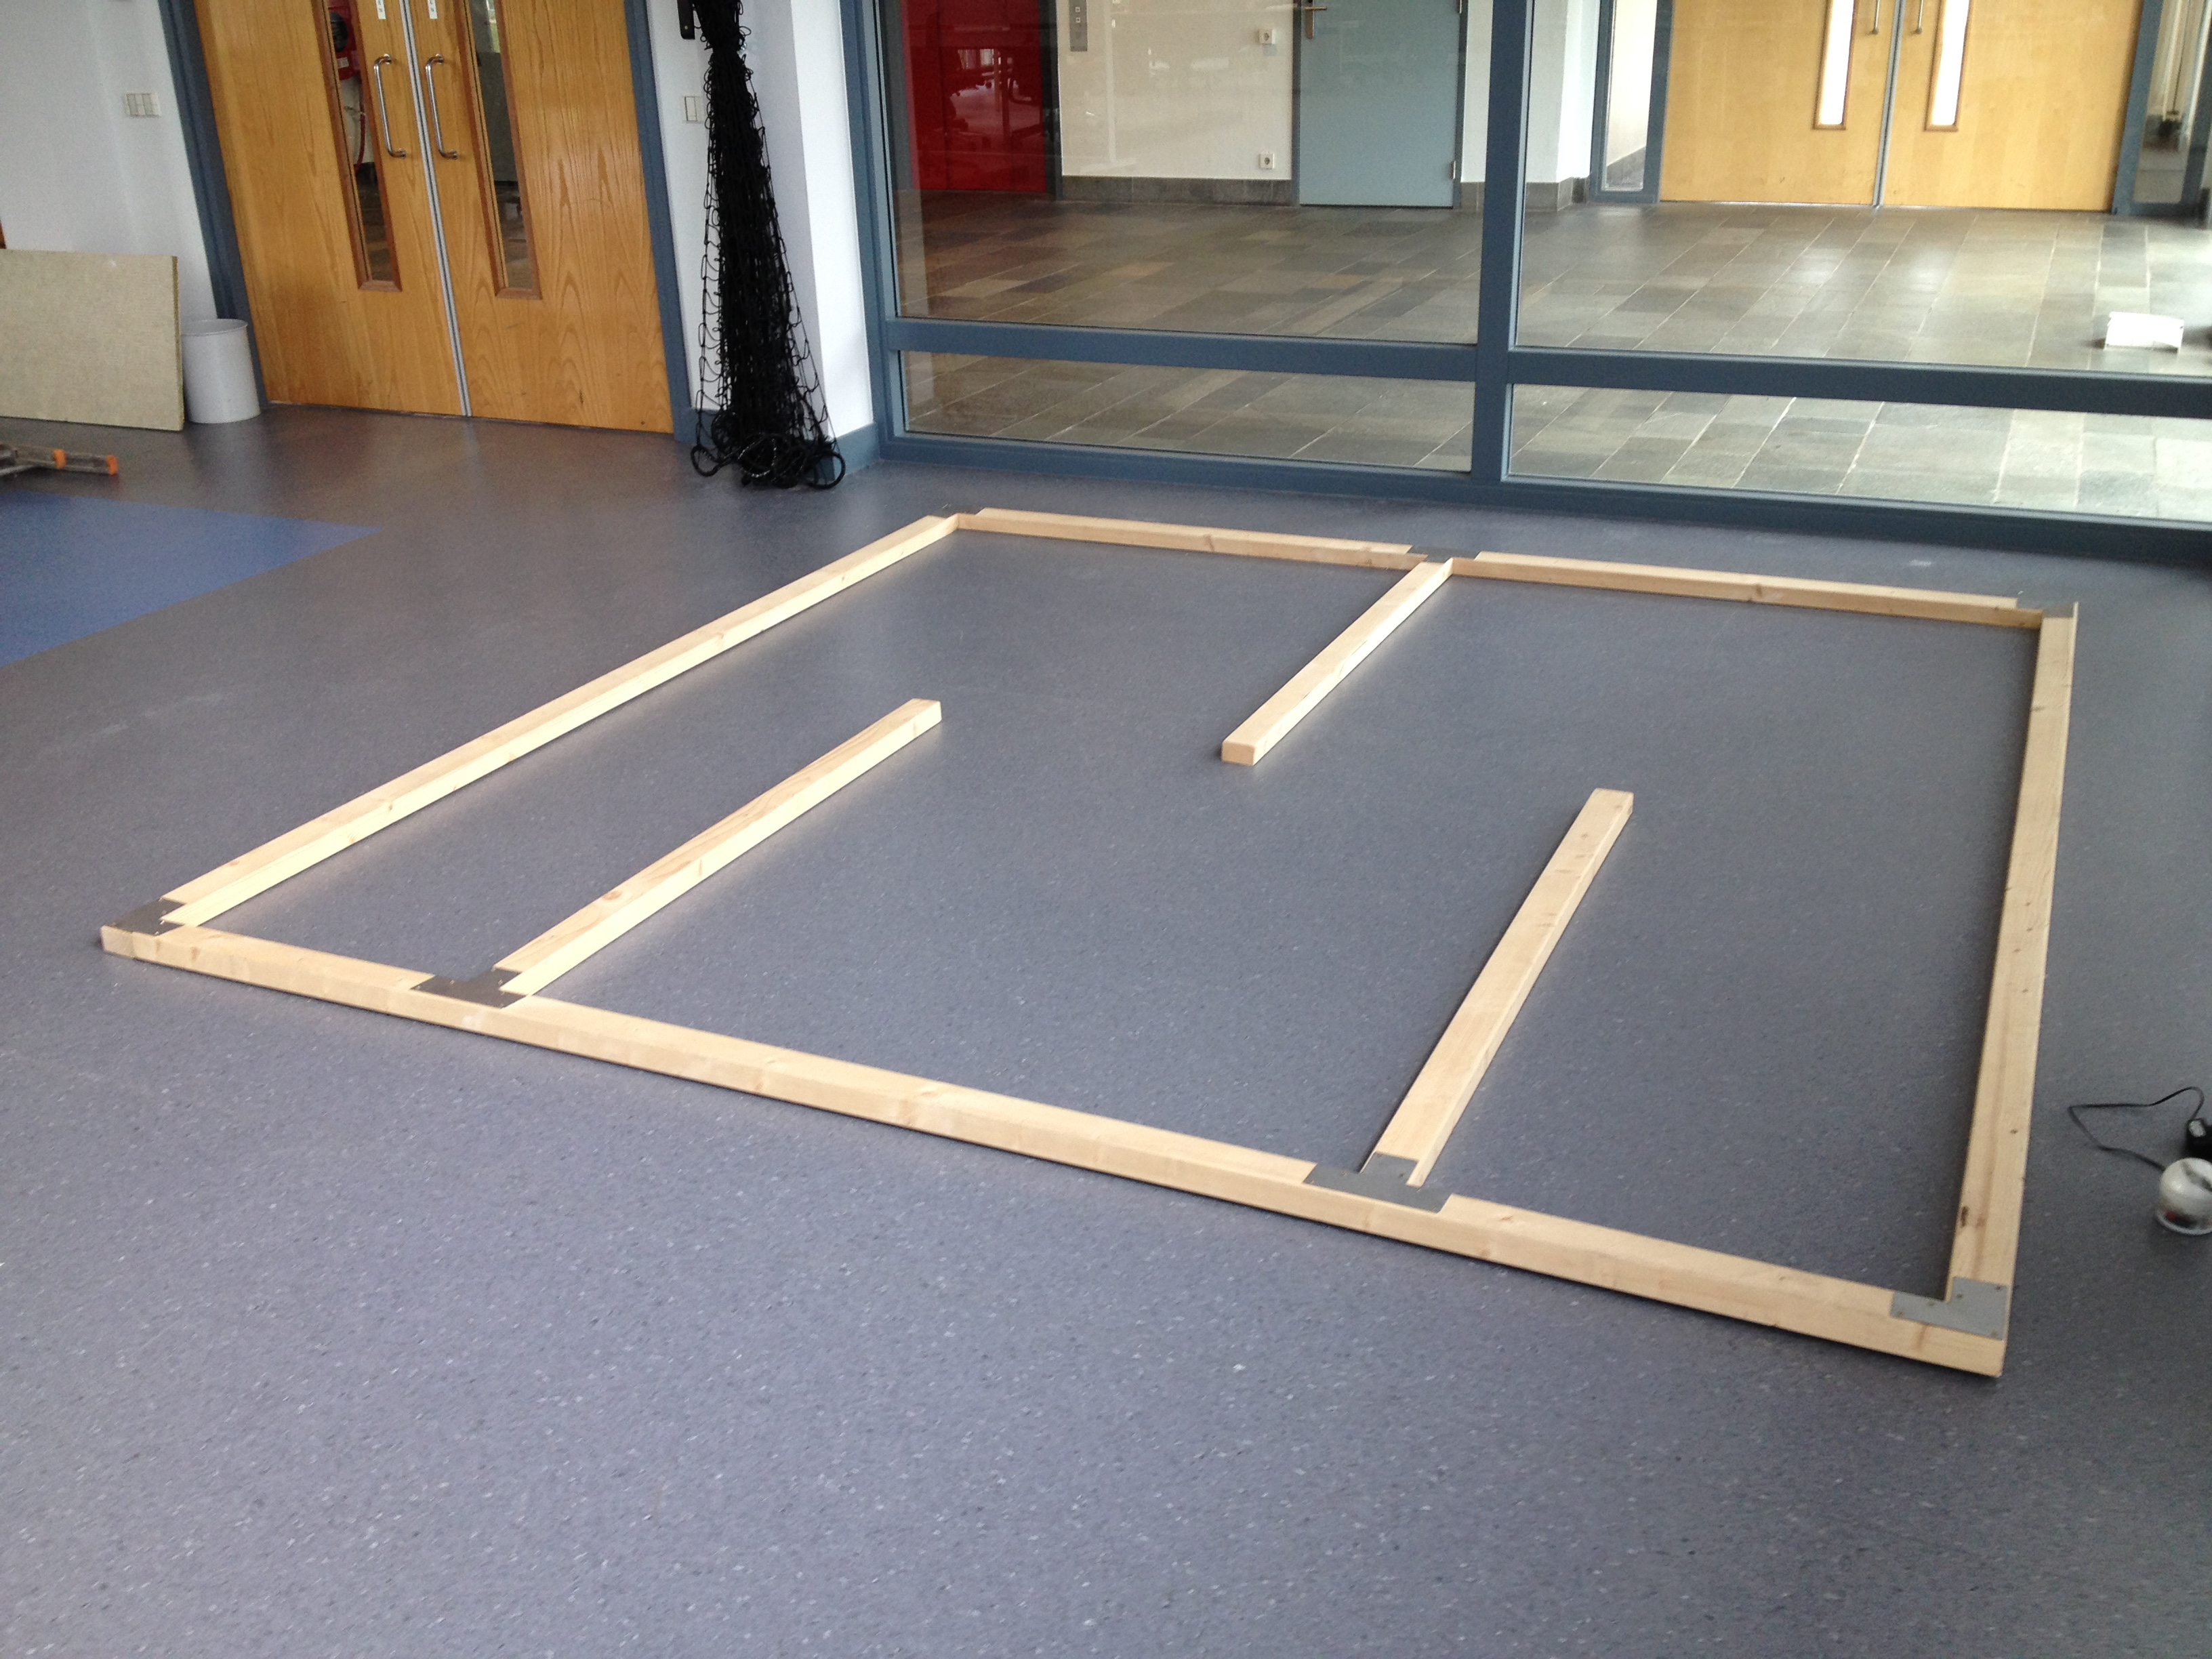
\includegraphics[scale=0.1]{./images/maze.jpg}
\caption[Real world environment for impact-based SLAM]{Real world environment for impact-based SLAM}
\label{maze}
\end{figure}

\begin{figure}
\centering
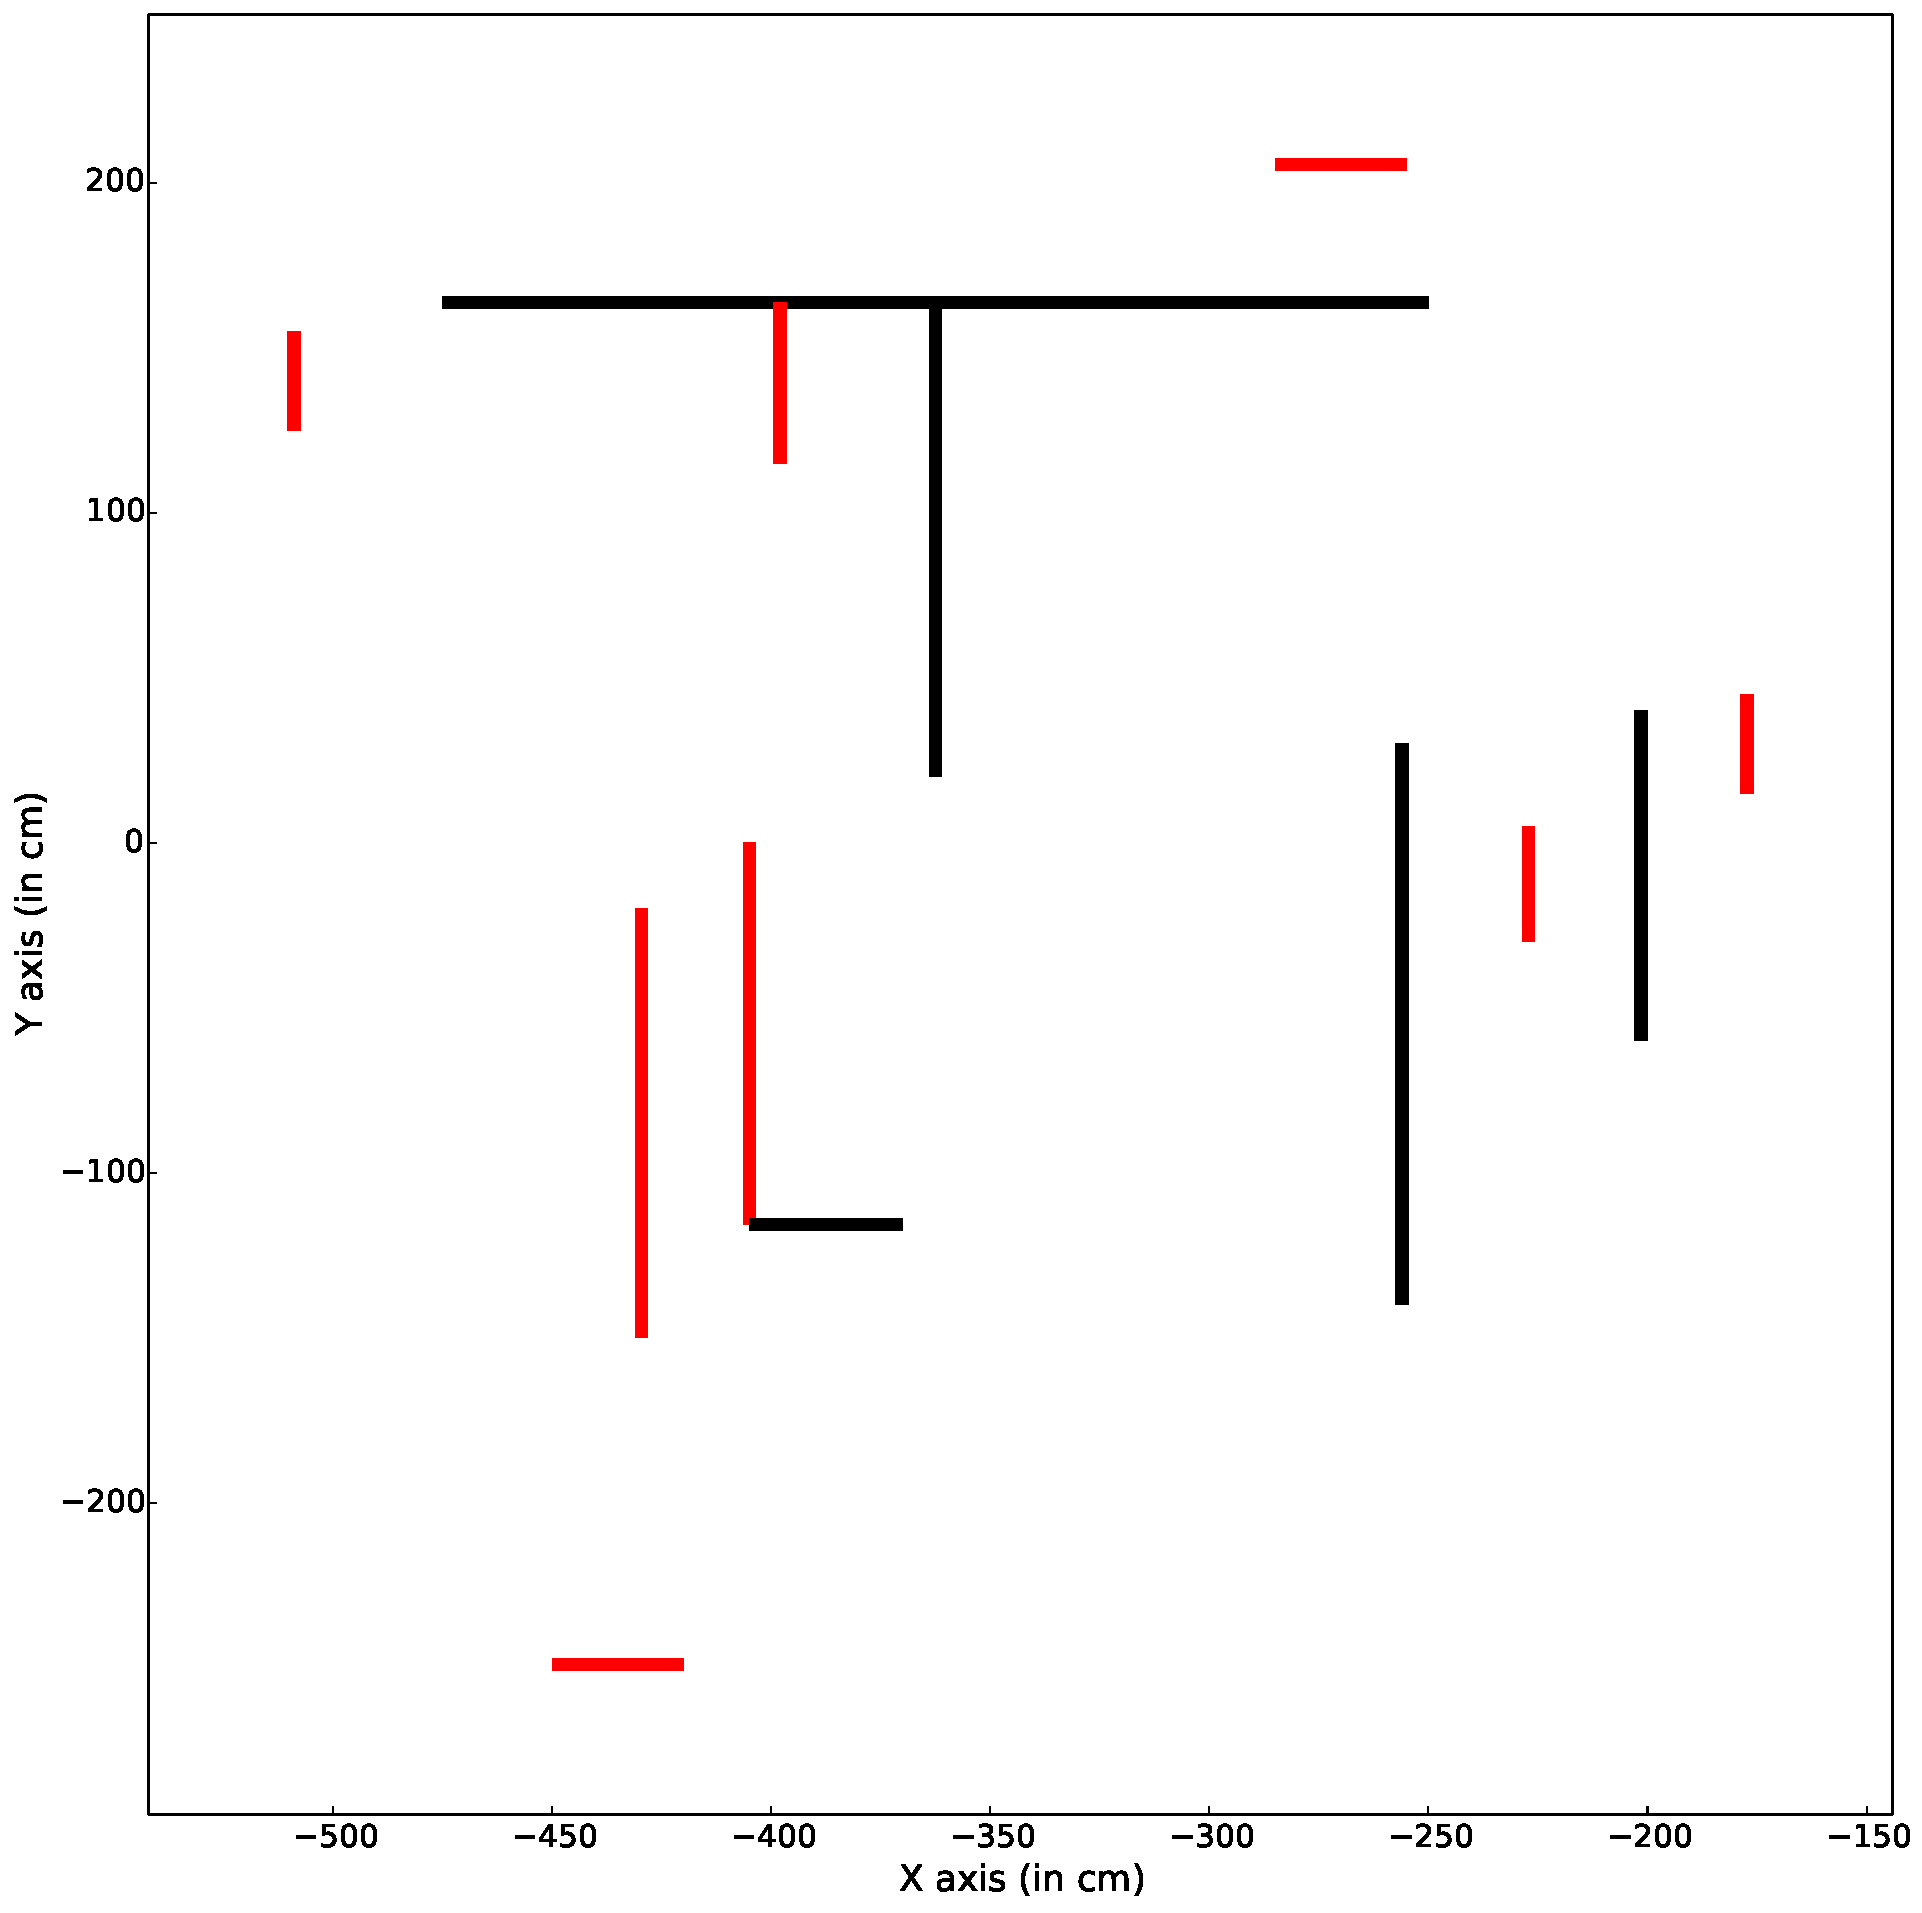
\includegraphics[scale=0.25]{./images/single_lcmap}
\caption{Output map of SLAM solution with constraint incorporation as measurement with low covariance. The red coloured landmarks are spurious and are not updated. The histogram distribution is processed finally and pruned to the nearest neighbouring landmarks.}
\label{single_lcmap}
\end{figure}

In the output map, the walls are orthogonal to each other and an initial local loop (upto neighbouring landmarks) closure is performed correctly for the robot starting from bottom-right corner of the maze. The initial local loop closures can be seen from the neighbouring landmarks that are accurately estimated (black coloured landmarks). The orthogonal constraints are added as measurements with a low covariance (close to zero) at every correction step through an additional EKF update \cite{rodriguez2007consistency}, \cite{newman1999structure}. This constrained estimation projects the prior estimate onto the constraint space which is same as projection operation in least squares framework. However, the approach yields inconsistent estimates here (as seen from the spurious landmark growth) due to lack of proper modelling of correlations between all the landmarks and robot. Inconsistency can also arise through linearization errors which is discussed in detail in \cite{rodriguez2007consistency} and \cite{julier2007using}.

In this thesis, landmarks are assumed to be independent (no cross-correlations) through Rao-Blackwellization which may not hold in structured environments. This is because the incoming measurements are correlated through the geometric structure of the environment apart from the robot pose error. The lack of maintaining these cross-correlations accurately is a key issue for inconsistency since an EKF update uses the correlations (covariance matrix) for updating the state estimate. As the correlations are modelled inaccurately, addition of constraint measurements with very low covariance can result in a large reduction in covariance which results in an inconsistent solution. The large reduction in covariance for landmark updates can be seen in Figure~\ref{landmark_wn}. Hence with few measurement (including constraint) updates, the covariance spuriously drops down or equivalently, the estimate becomes more certain. Hence, the later updates (no measurement updates after 600 iterations) does not contribute to any new information as seen from the lack of larger loop closures. The effect of correlations on the state estimate for the SLAM problem is asserted in Remark~\ref{rem_corr}.

\begin{figure}
\centering
\hspace*{-1cm}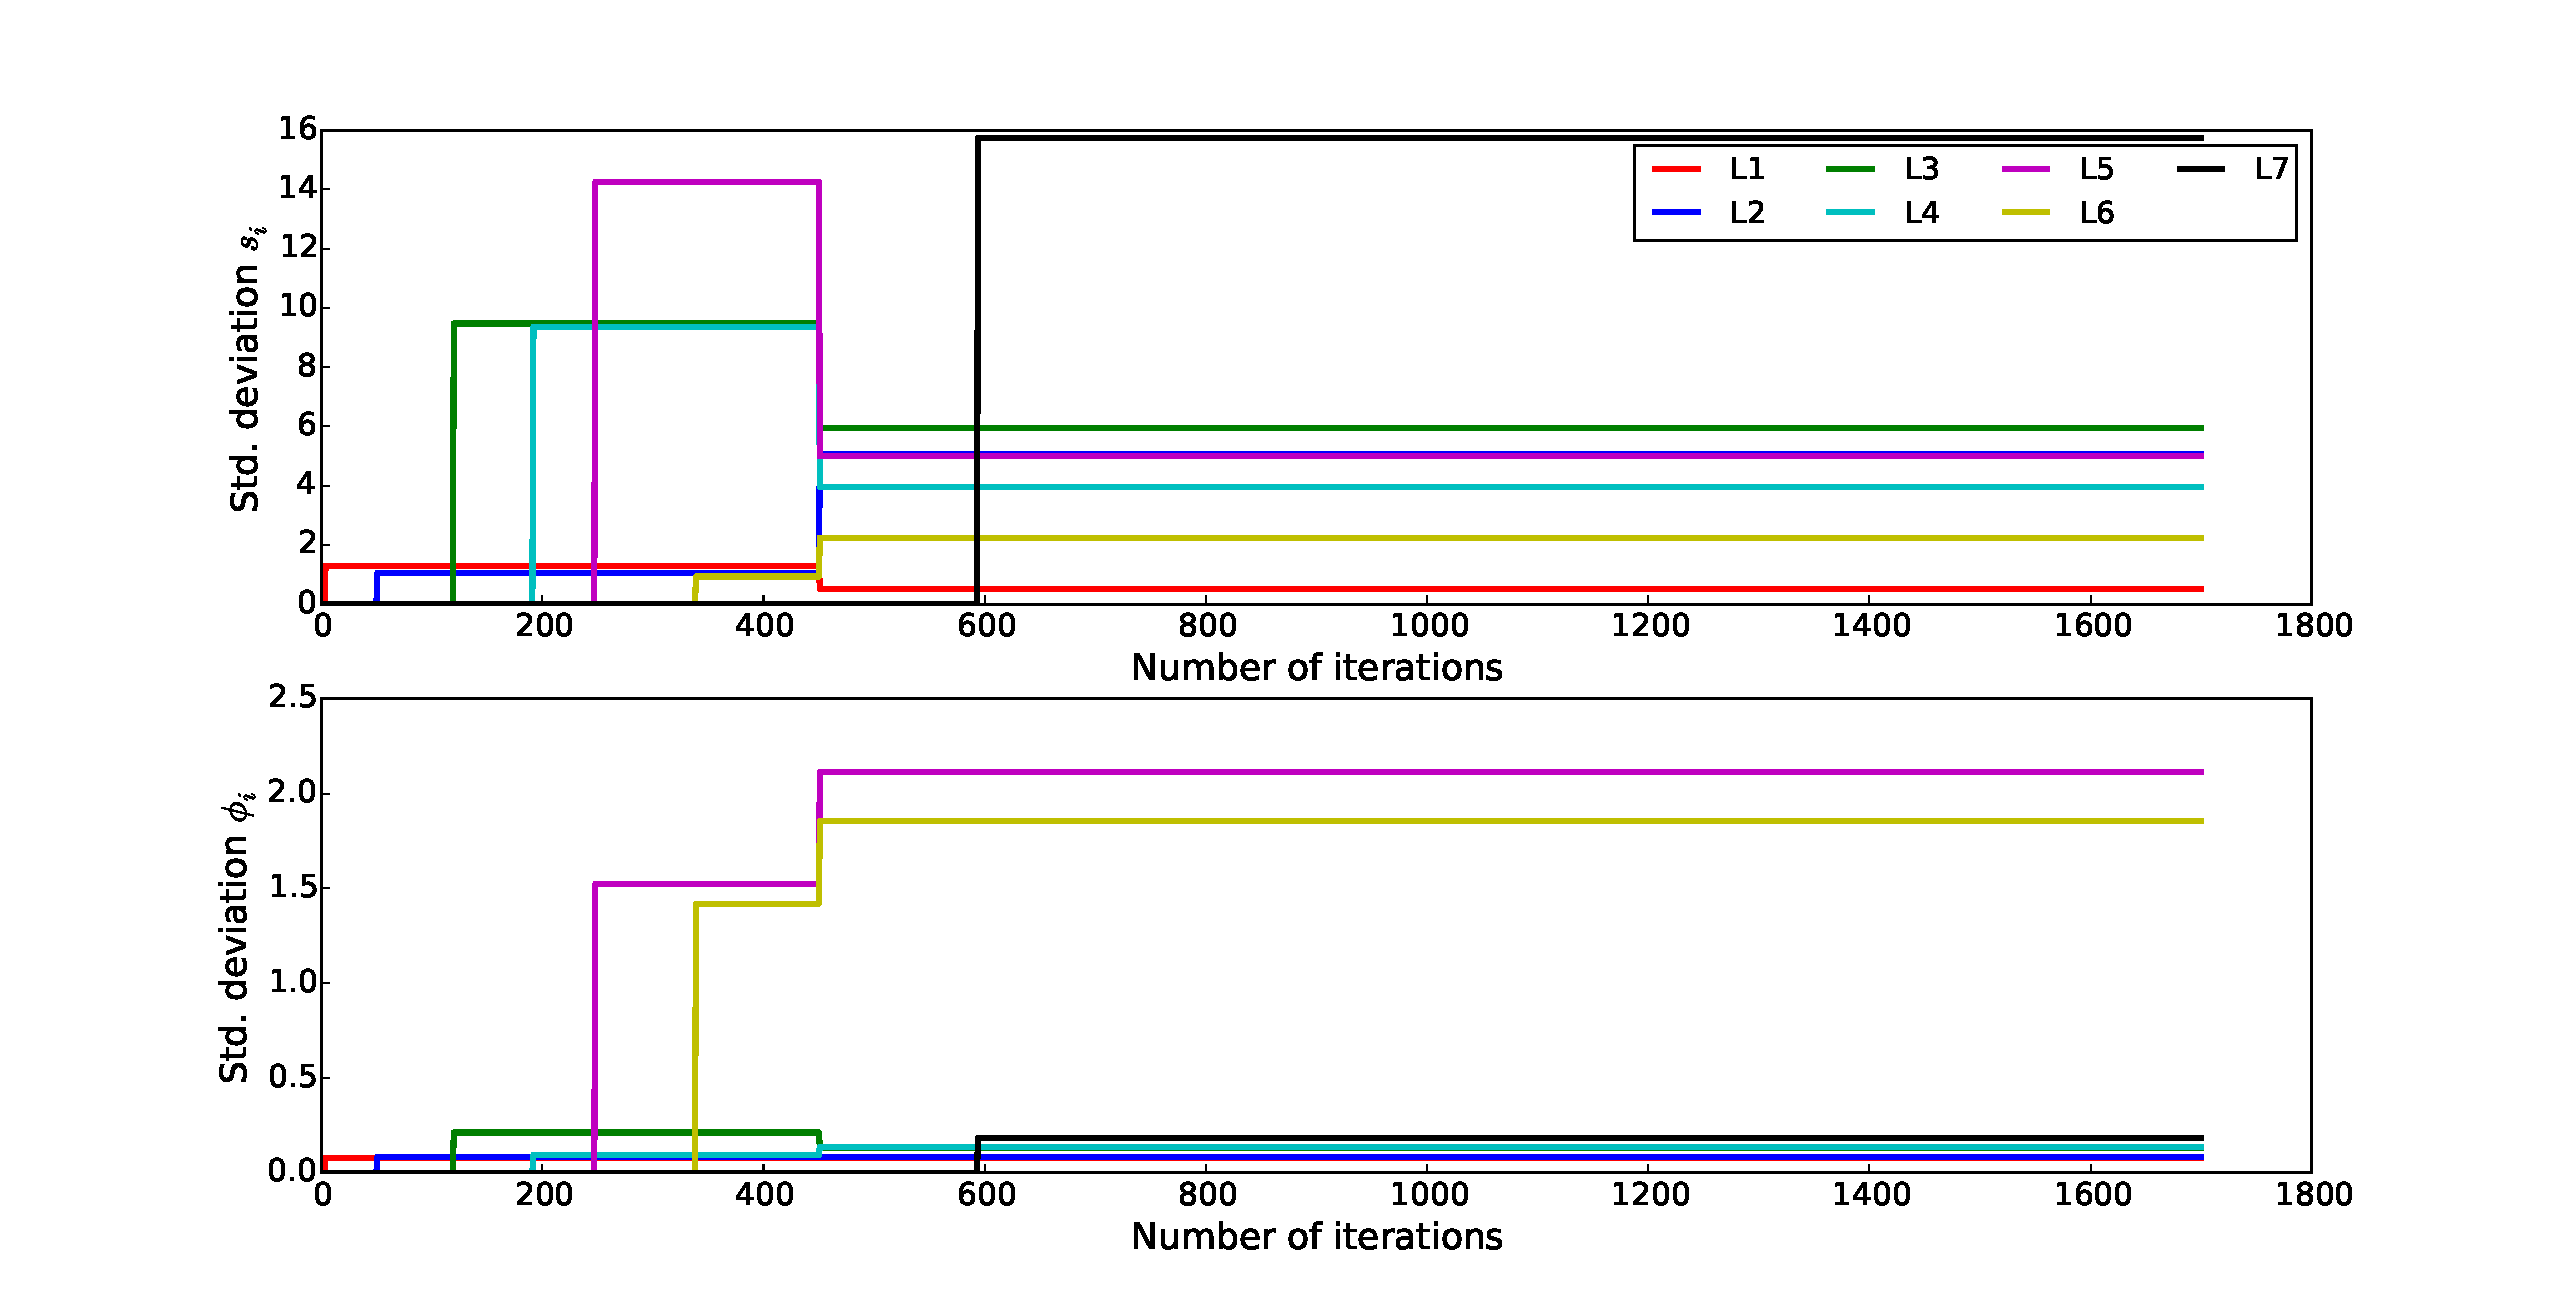
\includegraphics[scale=0.4]{./images/landmark_wn}
\caption[Convergence plot of the SLAM solution with constraint updates of low covariance]{Convergence plot of the SLAM solution with constraint updates of low (close to zero) covariance. The standard deviation ($1\sigma$) plots for the (along unit normal axis) position $s_i$ and orientation $\phi_i$ of landmarks are computed from the ML particle.}
\label{landmark_wn}
\end{figure}

\begin{rem}
For a small magnitude in cross-correlation between state estimates in SLAM, incoming measurements are treated with a higher novelty which updates covariance information spuriously. A large magnitude of cross-correlation results in a rigid covariance structure which makes an estimate more susceptible to error of other correlated estimates. 
\label{rem_corr}
\end{rem}

The loss of consistency can be seen from the Figure~\ref{single_lcmap} through lack of a large loop closure. This can also be seen through creation of spurious landmarks (a spurious local map) after traversal of a large loop. The spurious creation is due to formation of a new local map of the same region which was mapped long time back. 

The covariance of the state estimates with a low covariance constraint update is shown to converge to a bounded value as shown in Figure~\ref{landmark_wn}. It is observed that there are not much landmark updates since new spurious landmarks are created due to lack of a consistent estimation. As covariance $\Sigma$ drops down, past landmarks become more certain and data association gets affected. This is verified from Equation~\ref{da_pfslam} where magnitude of a likelihood to any measurement reduces as covariance drops down. This also holds for other state-of-the-art data association techniques based on associating measurements using covariance information. As data association gets poor, new landmarks are created for measurements with lower noise.

An effective approach for improving the consistency is through modelling the correlations using a single joint covariance estimate for all the landmarks (a single large covariance matrix for every particle in particle filter-SLAM) in the map and propagating it over the incoming measurements. The joint covariance maintains correlations due to geometric structure as well as the correlations introduced through robot pose error. However, the use of a joint covariance matrix involves higher computational complexity and storage requirements ($\mathcal{O}(M\cdot N^2)$ where $N$ is the number of landmarks in the map). Though conditional independence in landmark states through Rao-Blackwellization is lost due to the geometric correlations, higher consistency can be achieved at the expense of computational efficiency.

An alternative approach for ensuring consistency and at the same time exploiting the Rao-Blackwellized property is to update the constraints in a a conservative fashion using \acf{CI} where the landmark pose estimates are updated with the constraint measurements with a non-zero covariance. This approach does not take the cross-correlations into account but yields a consistent estimate. However with this approach, it is difficult to compute the constraint measurement covariance at every time step accounting for the loss of correlations. In the practical implementation, the covariance magnitude is chosen heuristically based on the current magnitude of orientation error.

The convergence to a more accurate solution is achieved using covariance intersection. The number of spurious landmarks are reduced since more loop closures (with a longer loop) are performed as seen from the updates. For impact-based SLAM with constraint updates using covariance intersection, the convergence plots are shown in Figures~\ref{landmark_cilc}~and~\ref{landmark_ci}. The convergence to a consistent solution shows the success of a SLAM solution.

\begin{figure}
\centering
\hspace*{-1cm}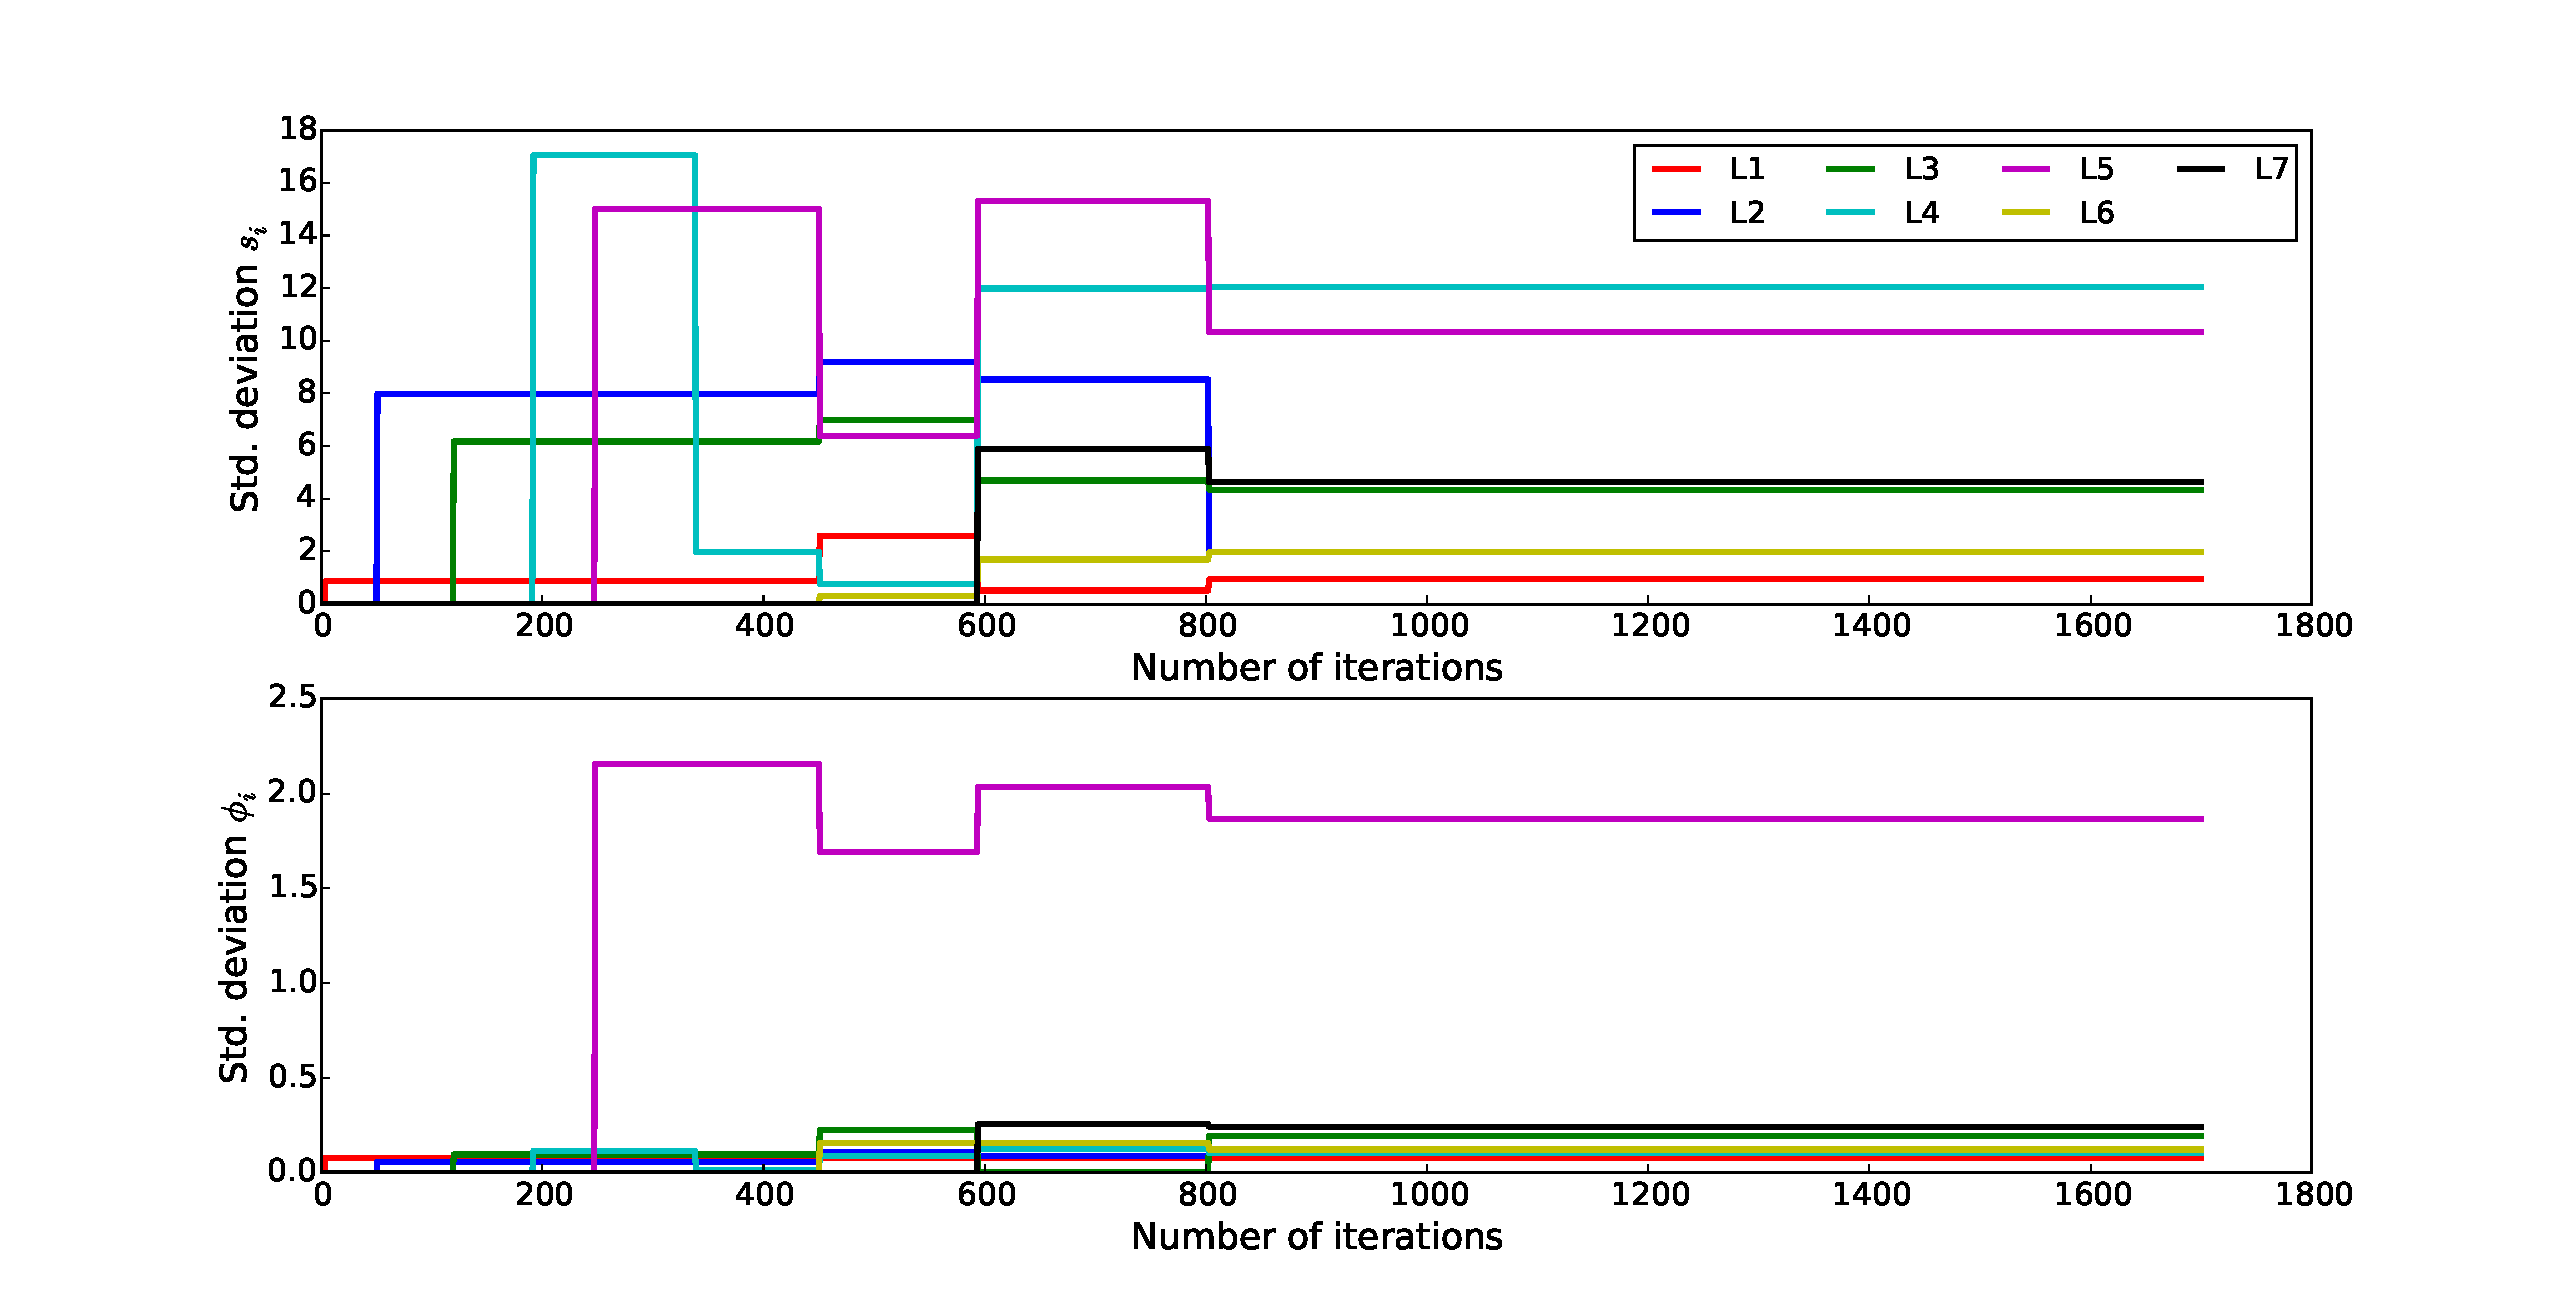
\includegraphics[scale=0.4]{./images/landmark_cilc}
\caption{Convergence in the map solution for a conservative constraint update of covariance $R_{CI}=0.1\cdot\Sigma_{\theta}$. The standard deviation ($1\sigma$) plots for the position $s_i$ and orientation $\phi_i$ of landmarks are computed from the ML particle.}
\label{landmark_cilc}
\end{figure}

\begin{figure}
\centering
\hspace*{-1cm}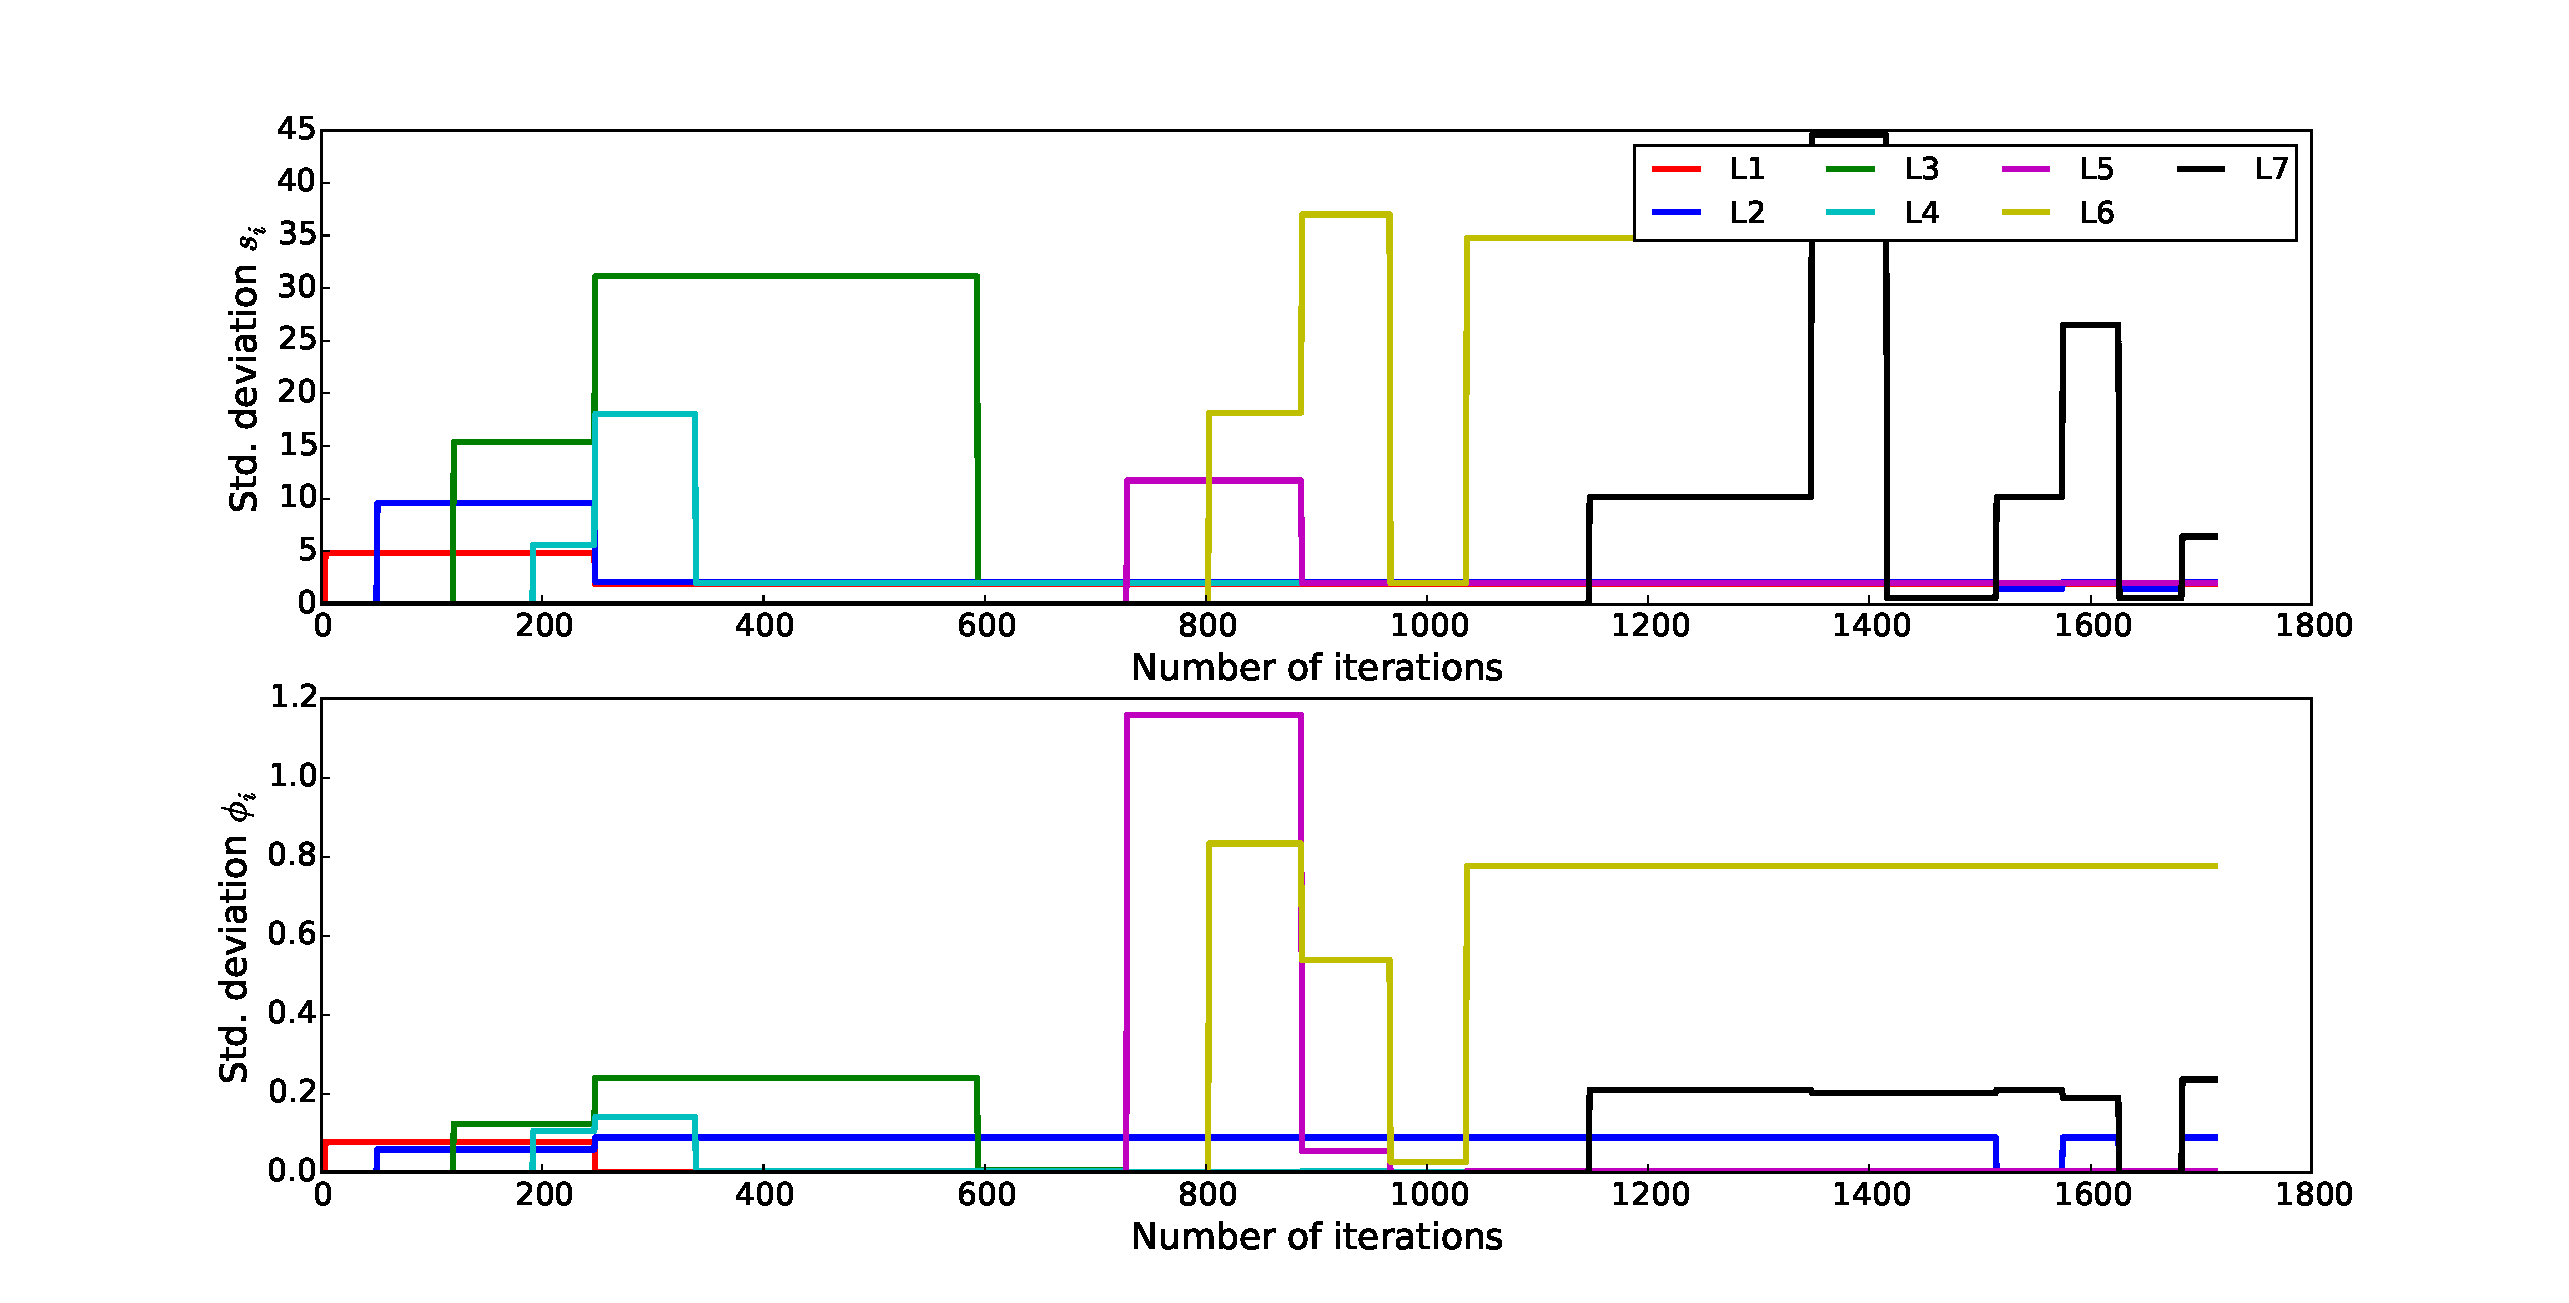
\includegraphics[scale=0.4]{./images/landmark_ci}
\caption{Convergence in the map solution for a conservative constraint update of covariance $R_{CI}=0.5\cdot\Sigma_{\theta}$. The standard deviation ($1\sigma$) plots for the position $s_i$ and orientation $\phi_i$ of landmarks are computed from the ML particle.}
\label{landmark_ci}
\end{figure}

\begin{rem}
The standard deviation (or covariance) increase is due to jumps between particles for plotting the most likelihood solution and the jumps are higher for a higher orientation error.
\end{rem}

The resulting output map of SLAM using the conservative constraint update is shown in Figure~\ref{single_map}. The conservative approach using CI results in a solution with a higher consistency as seen from the reduced growth of spurious landmarks. It can also be seen from Figure~\ref{landmark_ci} that landmarks are updated more frequently which suggests that better loop closures are achieved. Problems arising from bigger loop closure can only addressed with much better data association techniques such as \acf{JCBB} where multiple landmarks are considered simultaneously for association based on incoming measurements. The problem with impact-based SLAM is the lack of dense measurements from the environment and hence for considering Joint Compatibility, past subset of measurements have to be incorporated at every update step. 
 
\begin{figure}
\centering
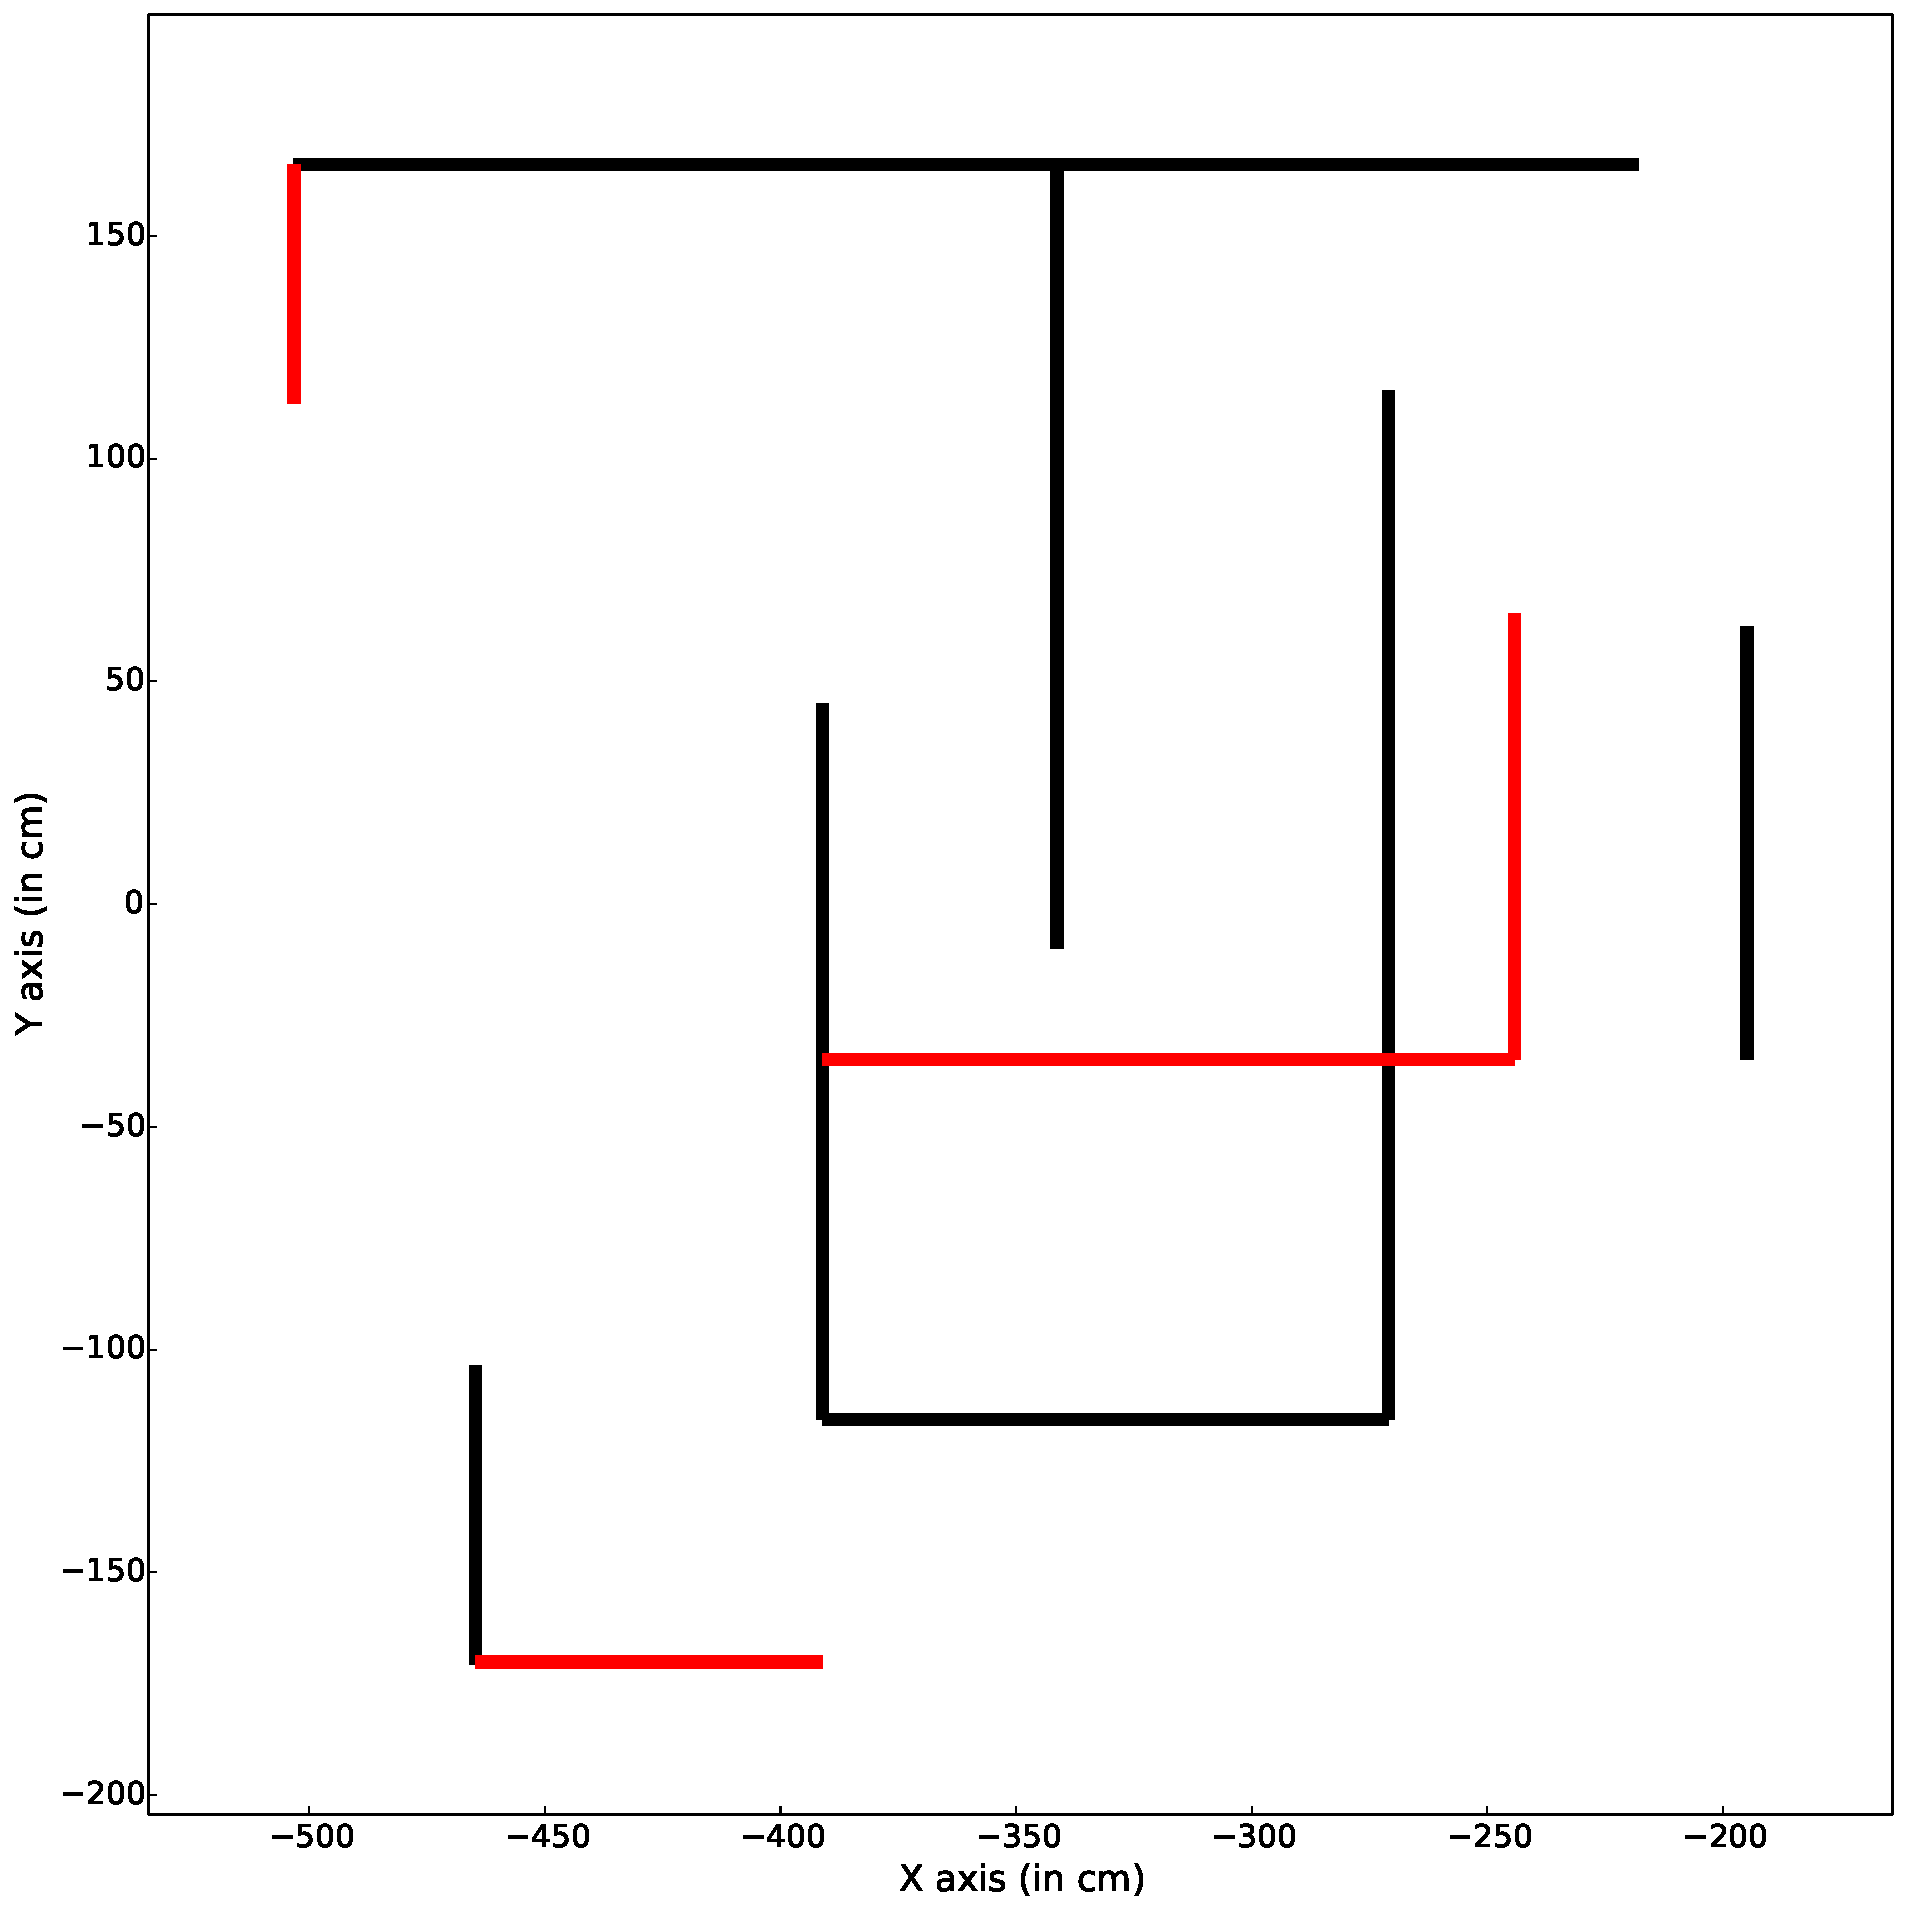
\includegraphics[scale=0.25]{./images/single_map}
\caption[Output map from a conservative SLAM solution using a single robot]{Output map from a conservative SLAM solution using a single robot corresponding to constraint measurement covariance of $R_{CI}=0.5\cdot\Sigma_{\theta}$. The red coloured landmarks are spurious landmarks initialized due to high motion error or false positives in collision. The histogram distribution is processed finally and pruned to the nearest neighbouring landmarks.}
\label{single_map}
\end{figure} 

An additional conservative update is carried out to account for the partiality in uncertainty update in a rectilinear environment. In a corridor environment, the covariance gets selectively updated along the direction of unit normal to the wall (or along the corridor width) while the covariance along the wall (or corridor path) increases due to process noise. This can be seen in Figure~\ref{ex1_scalepointlandmark} where error along the corridor gets accumulated until orthogonal information is available through a loop closure of a wall orthogonal to the corridor. This issue arises from the geometric structure of the environment and may be severe in environments with long corridors. As the landmarks are made independent through Rao-Blackwellization, a CI update is carried out between neighbouring orthogonal landmarks once a loop closure is achieved along the orthogonal direction. This update also helps in an accurate histogram update since the histogram update is influenced by the covariance of the landmark position (coordinate axis along the wall).

The histograms of landmarks are pruned to the nearest neighbours and the histograms along the perimeter are pruned based on environment size assumption. The discretization or rasterization level of histograms depends upon minimum wall opening (such as doors) assumption to speed up robot exploration. A key advantage about using histogram maps is collinear consistency of the output map which is not present in other map representations such as point landmarks and occupancy maps.

Other issues related to the practical impact-based SLAM are false positives generated by Sphero and corner collisions. The false positive detections of Sphero collision is reduced by increasing the impact threshold (rate of acceleration) on the accelerometer axes. In addition, a more effective way to reduce false positives is through a postponed association where landmarks are included in the map only if they are detected more than certain times. Few ambiguous collisions can occur when the robot hits a corner and such measurements are not considered in the estimation.

\section{Multiple robot SLAM}	\label{sec::map_merge}
The impact-based SLAM can be extended to multiple robots as a map-merging problem where individual maps are collected and merged at a point when a match is found. The histograms are matched using simple map comparisons with the assumption of environment size and approximate initial starting points of the robots. In addition to the map-merging, the assumptions are also used to prune length of histogram much similar to the single robot scenario.

With use of multiple robots for exploration, the merged-map is more consistent than single robot-SLAM since local maps are subjected to lower linearization errors. The effect of inconsistency through lack of accurate correlations is less observed in multiple robot scenario since local maps have lower number of updates but for generality, covariance intersection technique for constraint measurements is followed. Usually, multiple robots achieve faster exploration compared to a single robot exploration with a higher consistency. This can be seen in Figure~\ref{mmap3} through reduction in spurious landmarks

Covariance intersection is used for fusing the estimates of the intersecting (common) landmarks of the local maps and their histogram data is merged. For example, let $(x_1, P_1)$ and $(x_2, P_2)$ be the estimates of an intersecting landmark from the local map of robot 1 and 2 respectively. The merged estimate is found according to the following equations,
\begin{align}
x_{CI}&=P_{CI}\left(\omega\cdot P^{-1}_1x_1+(1-\omega)\cdot P^{-1}_2x_2\right) \\
P_{CI}&=\left(\omega\cdot P^{-1}_1+(1-\omega)\cdot P_2^{-1}\right)^{-1} 
\end{align} 
where $\omega$ is obtained by solving the following optimization using Golden Section search technique.
\begin{equation}
\min_{\omega} tr\left(\omega\cdot P^{-1}_1+(1-\omega)\cdot P_2^{-1}\right)^{-1}
\end{equation}

The output maps generated by two robots exploring the same environment are shown in Figures~\ref{mmap1}~and~\ref{mmap2}. The two maps closely represent the actual environment as shown in Figure~\ref{mmap3} and must be merged ($\mathcal{O}(1)$ complexity) consistently. The merged map is shown in Figure~\ref{mmap4} with histograms merged as well. An intersecting landmark pose has to be common among both the maps for fusion. It can be seen that local consistency is quite good from the convergence as well as the reduced number of spurious landmarks. However, the merged map is globally less consistent as seen from the unequal corridor width since the local maps of the robot are not correlated with each other. A possible approach (future work) to improve the global consistency is through continued exchange of particle information (fusion of two point clouds) during exploration between the robots. 

\begin{figure}
\centering
\begin{subfigure}{0.49\textwidth}
\centering
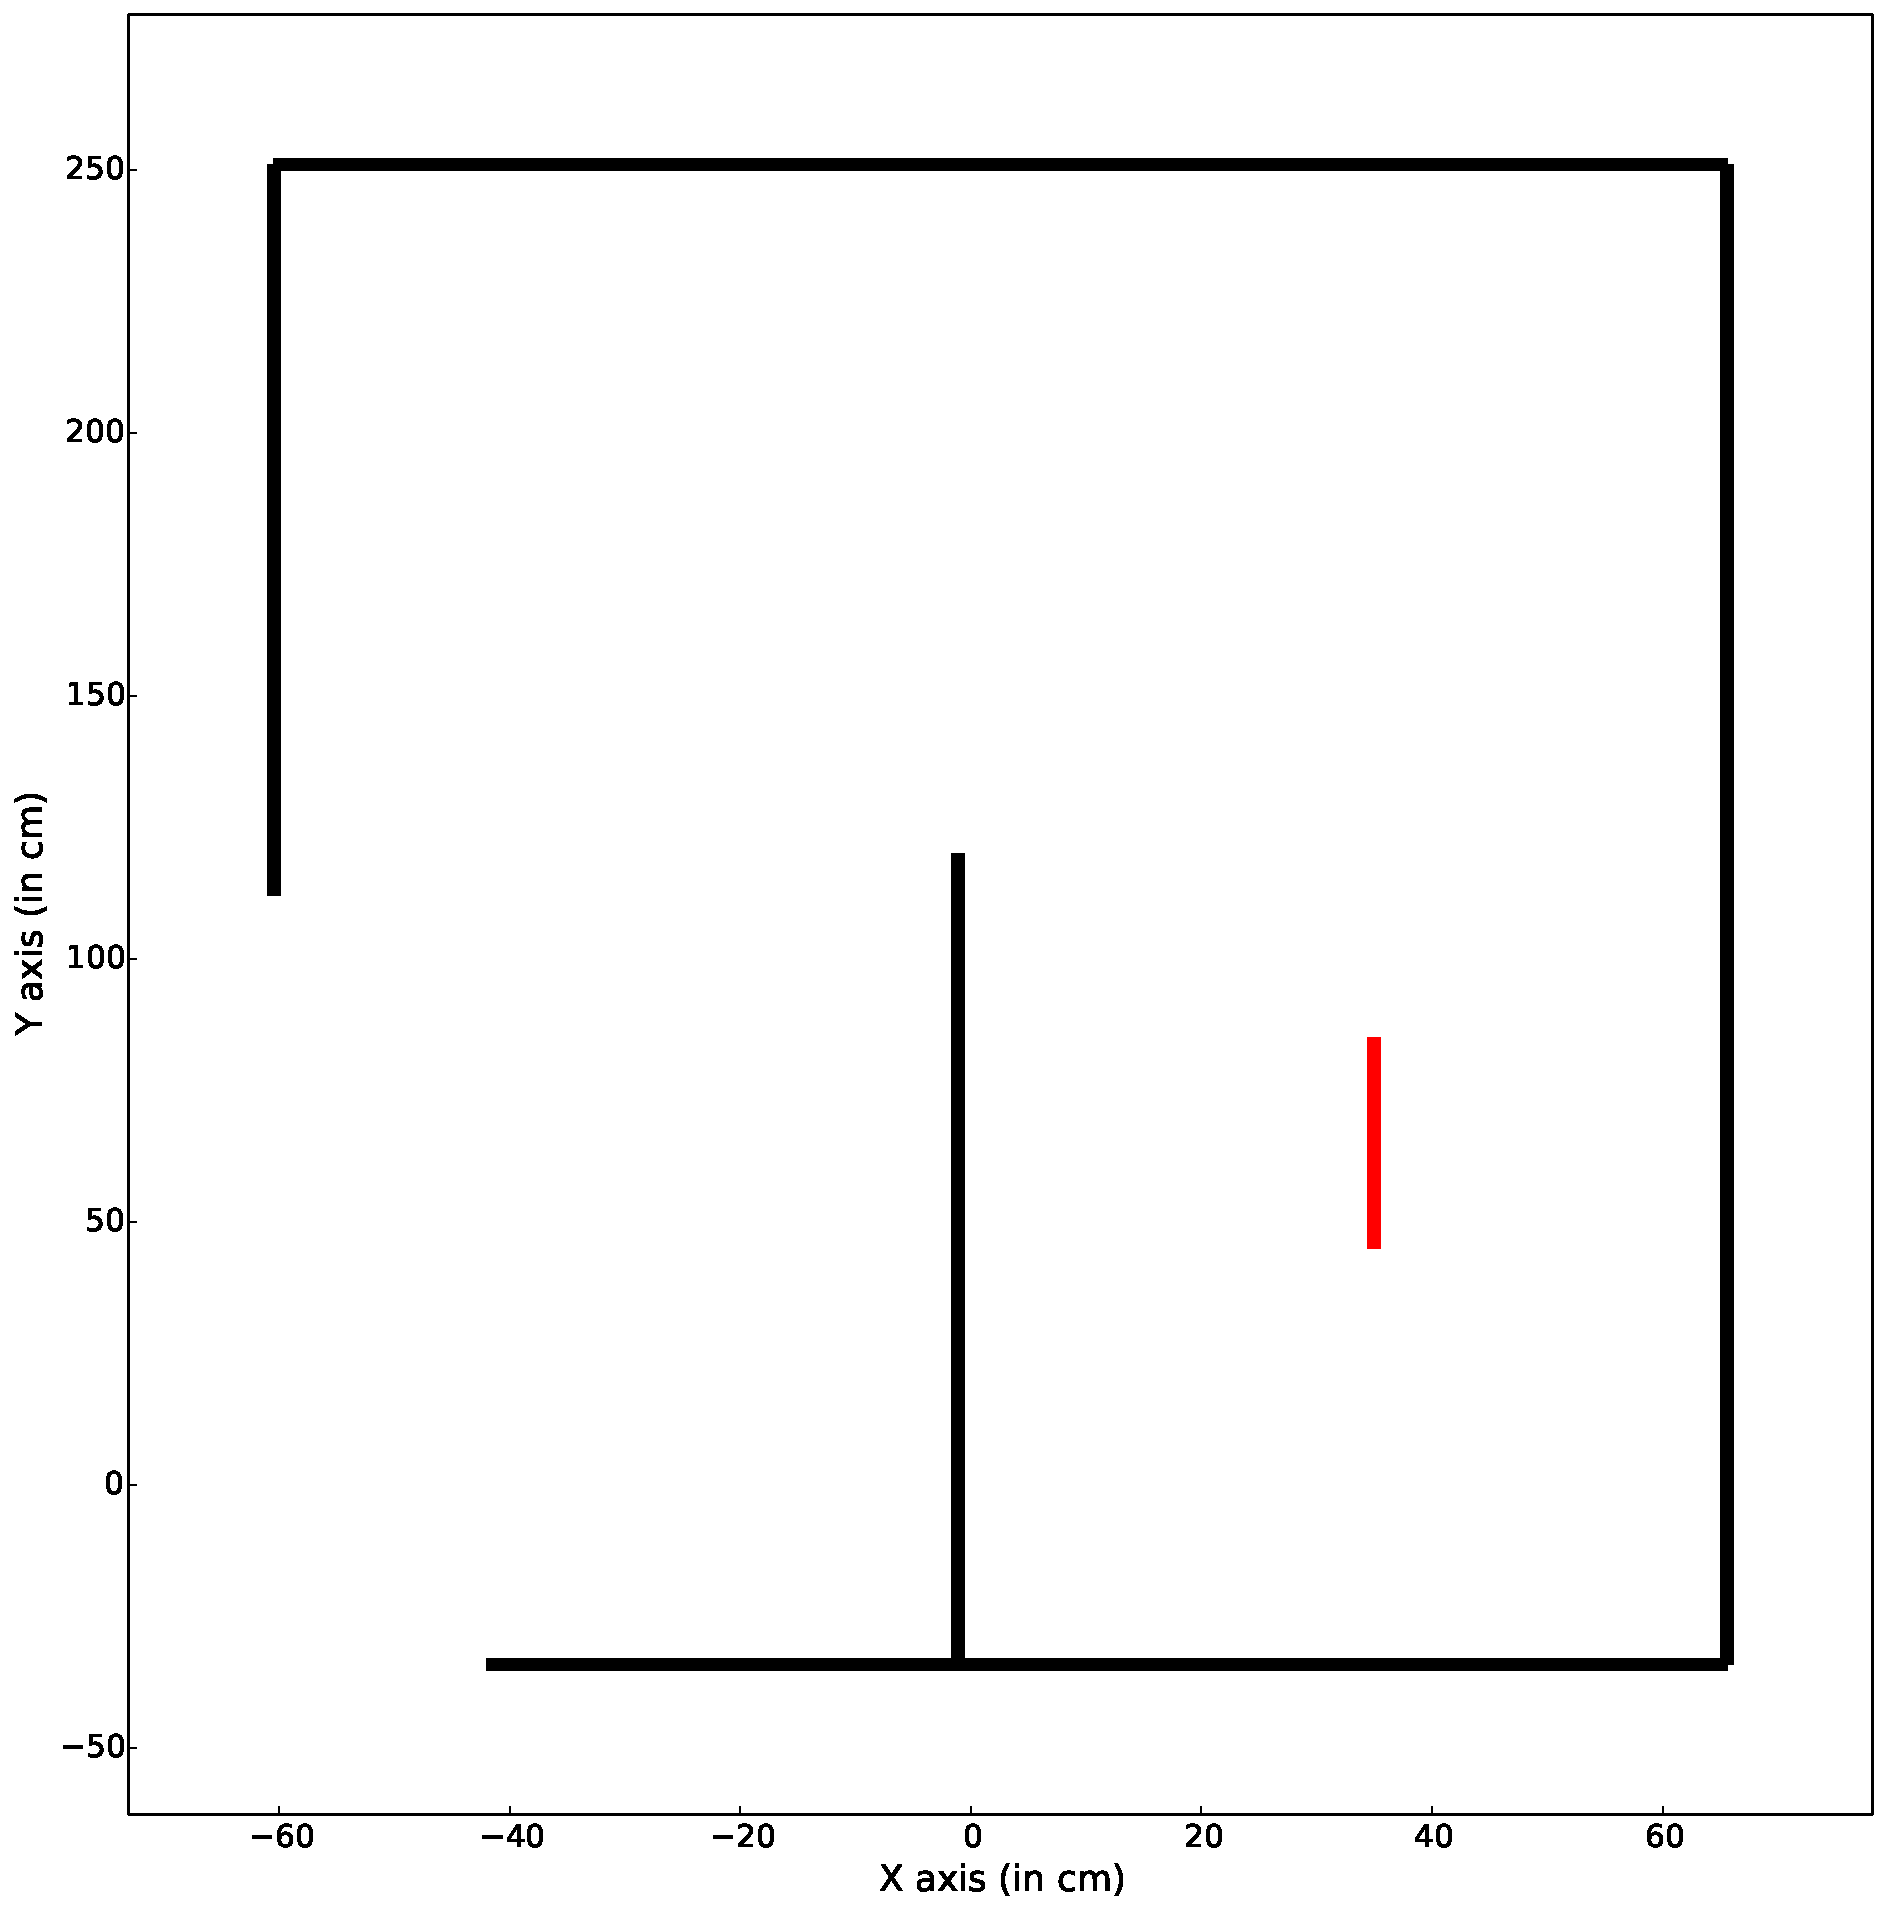
\includegraphics[scale=0.2]{./images/mmap1}
\caption[Local map generated by robot 1]{Local map generated by robot 1. The red landmark denotes a spurious landmark}
\label{mmap1}
\end{subfigure}
\begin{subfigure}{0.49\textwidth}
\centering
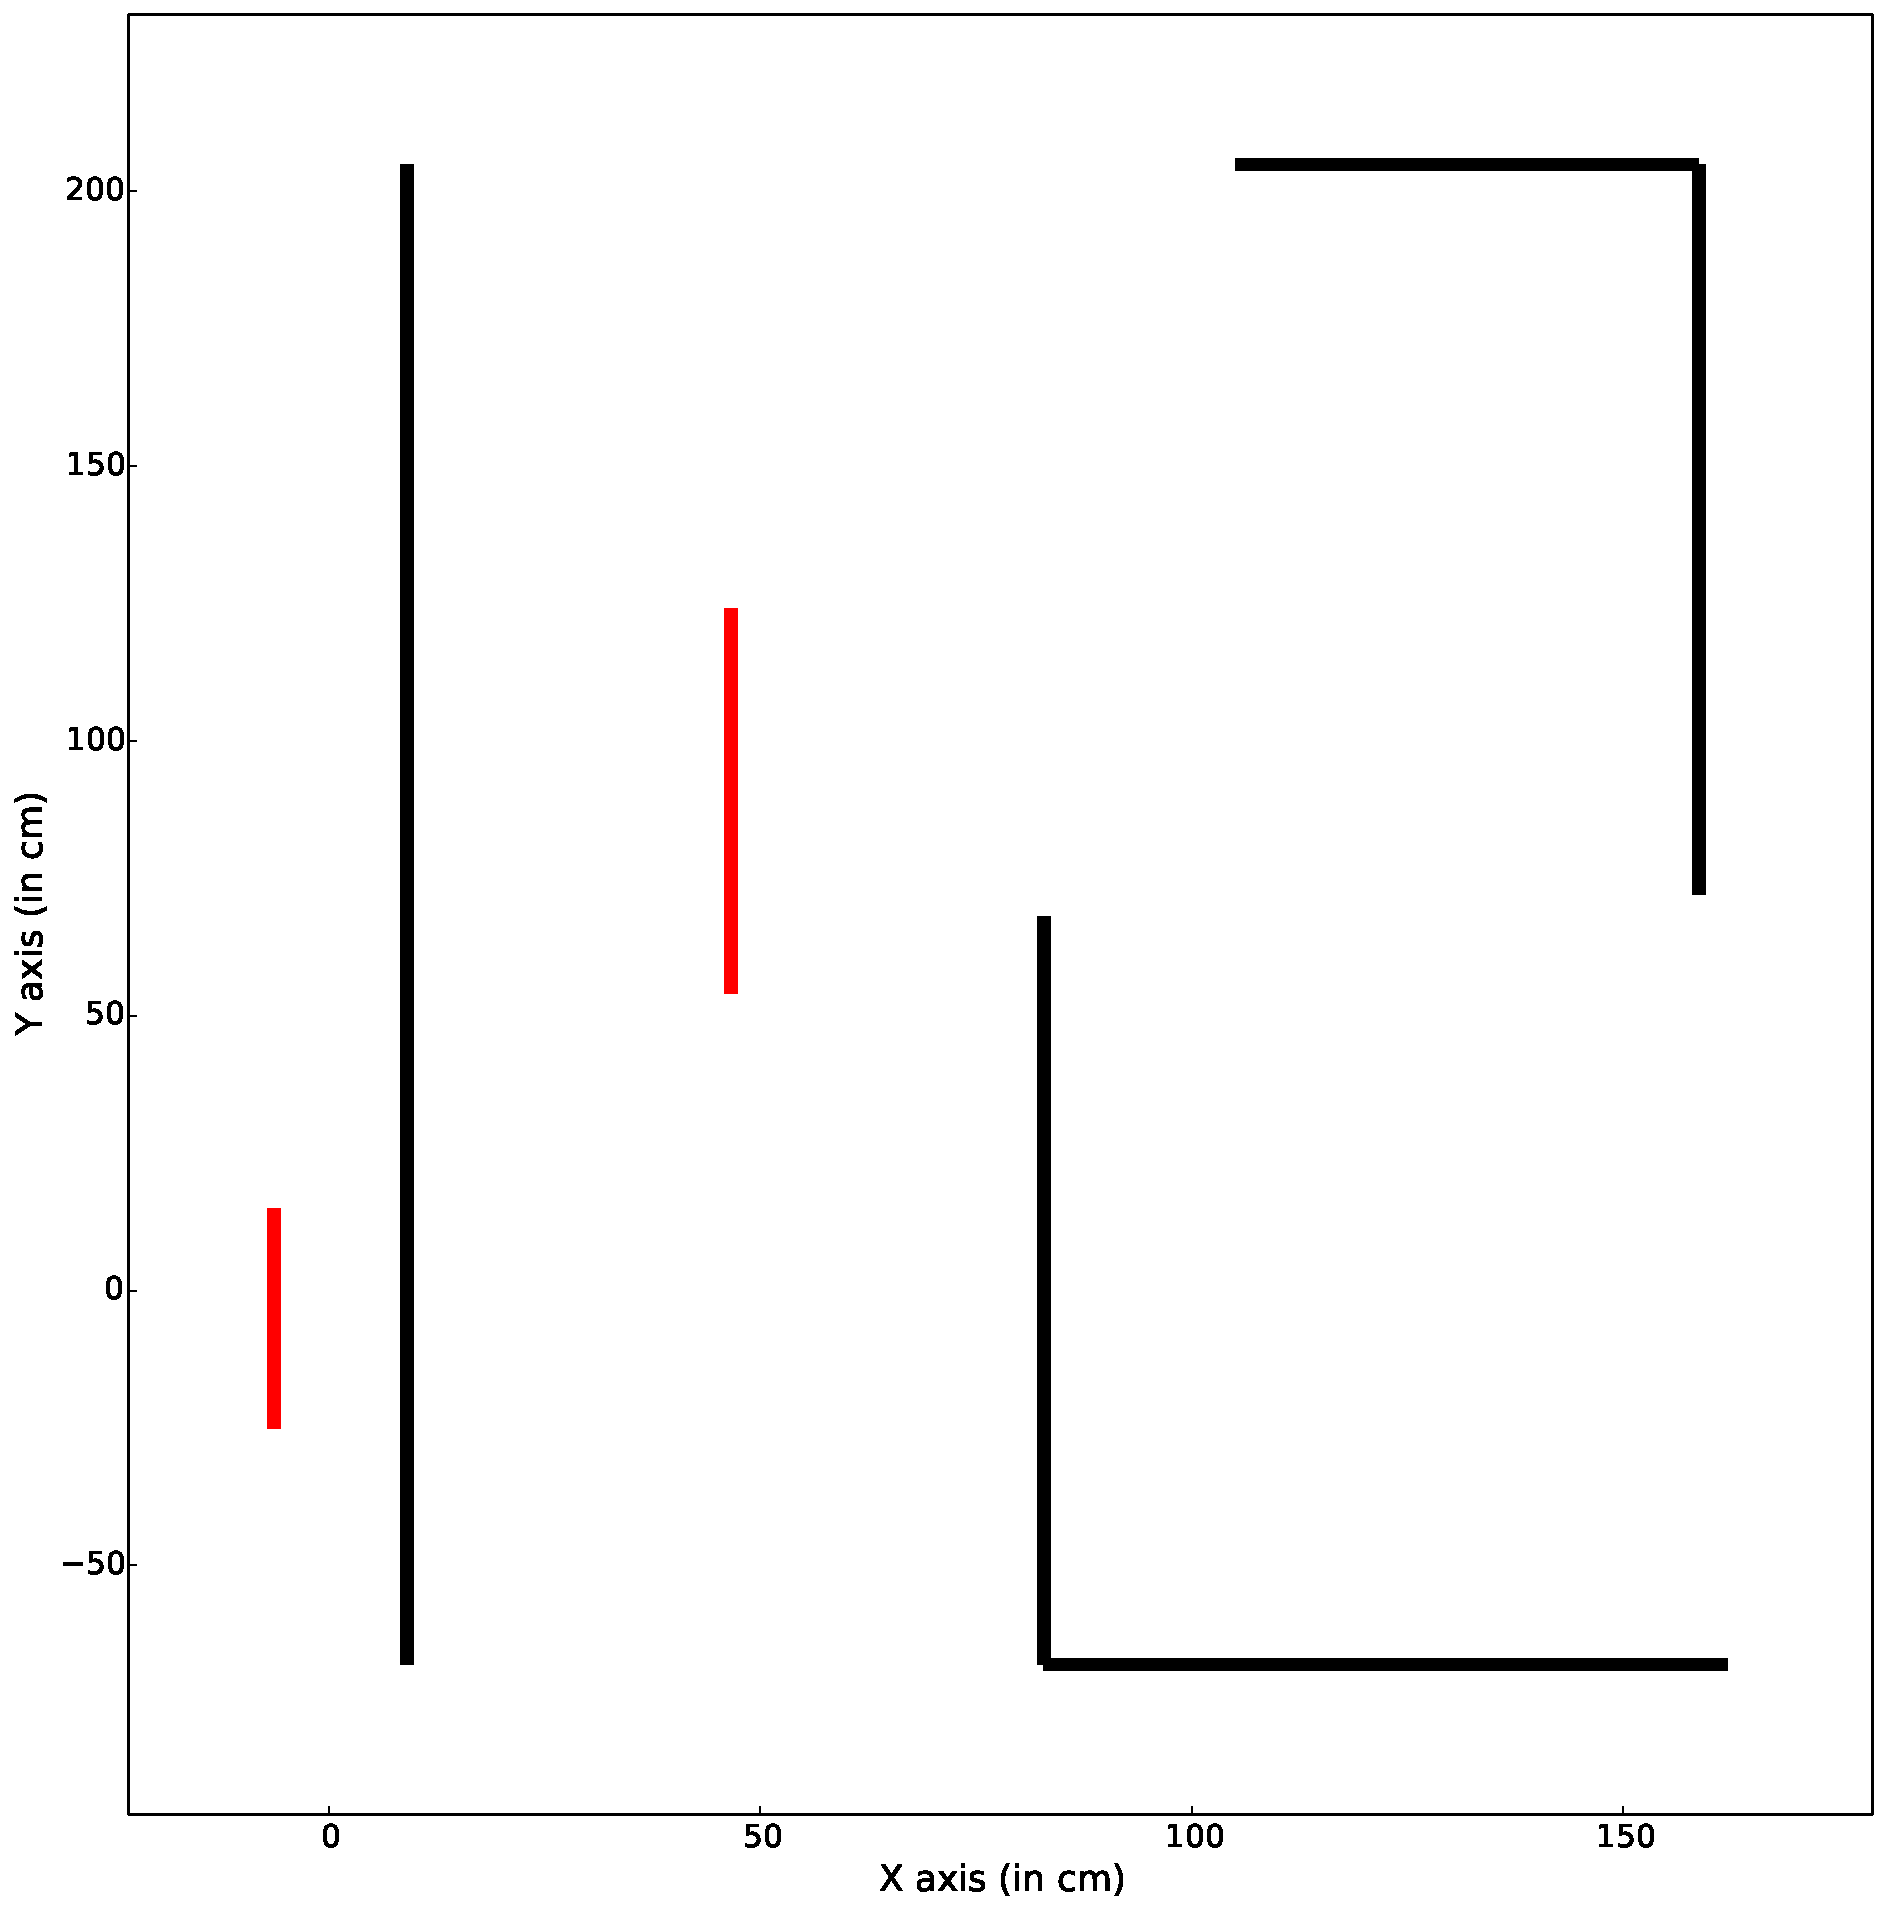
\includegraphics[scale=0.2]{./images/mmap2}
\caption[Local map generated by robot 2]{Local map generated by robot 2. The red landmarks denote spurious landmarks}
\label{mmap2}
\end{subfigure}
\end{figure}

\begin{figure}
\centering
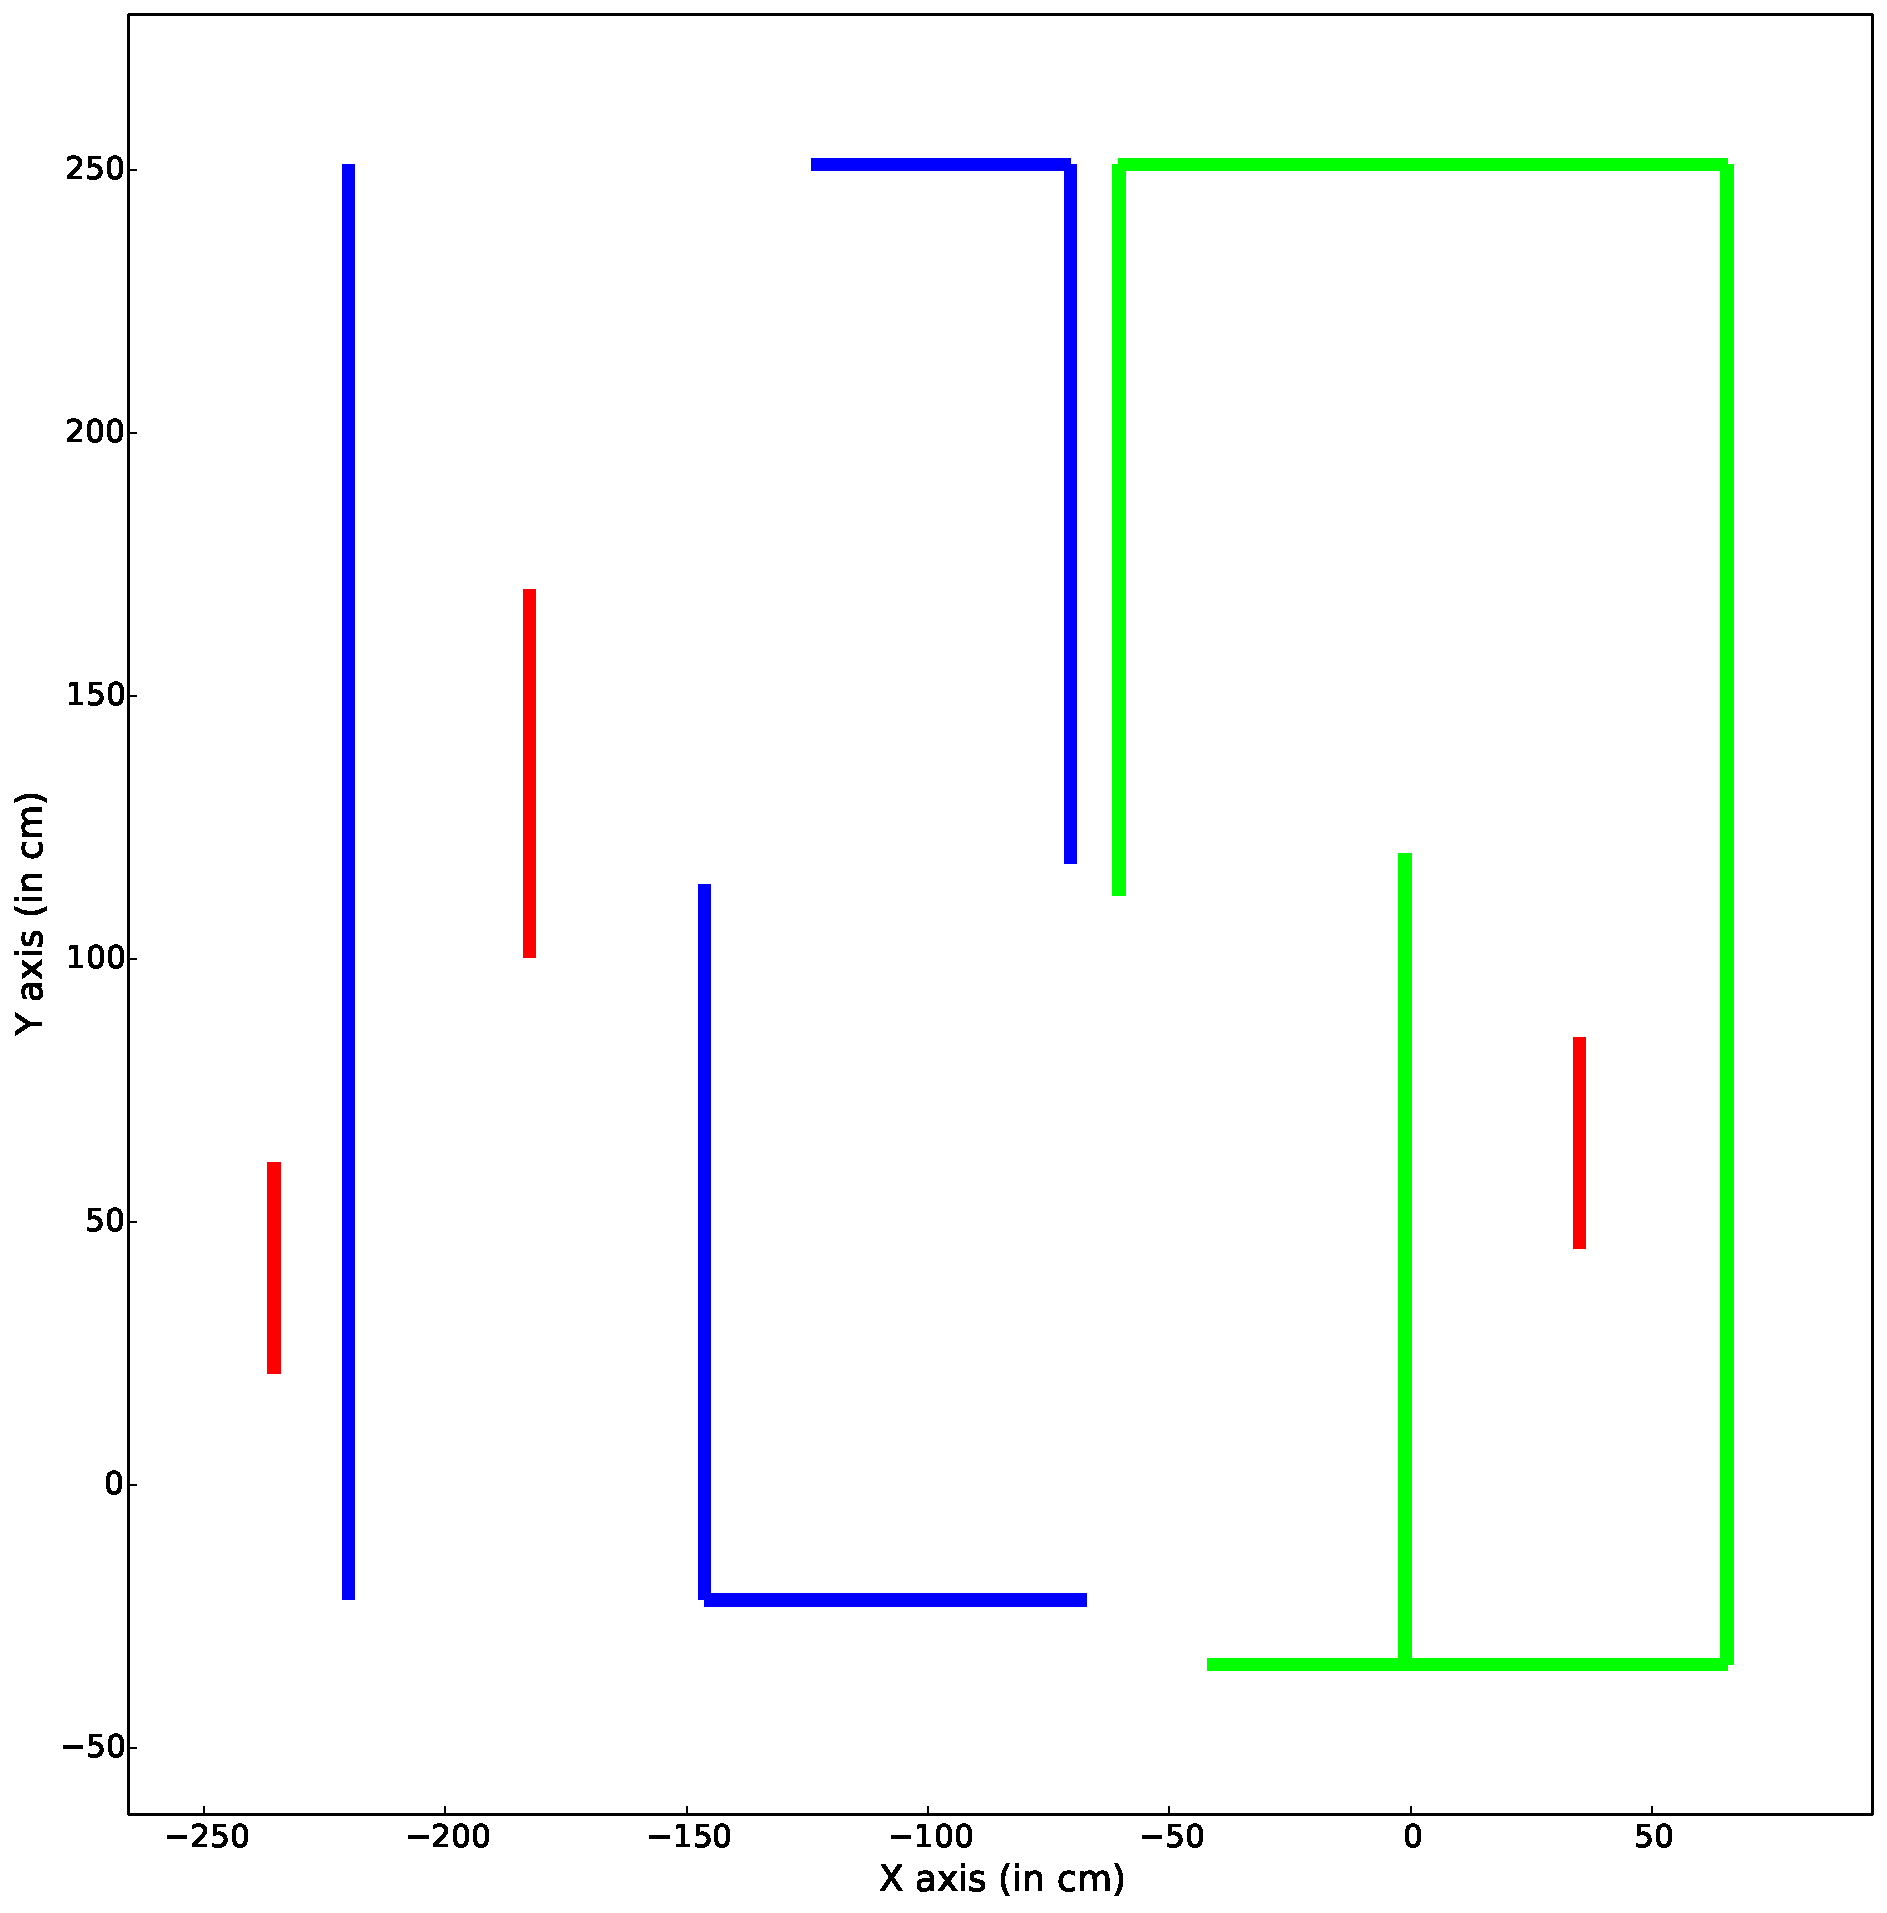
\includegraphics[scale=0.25]{./images/mmap3}
\caption[Map comparisons from the two robots ]{Local maps generated by the two robots. Each local map is denoted either by red or green color and the red landmarks correspond to spurious landmarks. Note that top horizontal landmarks of both the maps are pinned together for comparison.}
\label{mmap3}
\end{figure}

\begin{figure}
\centering
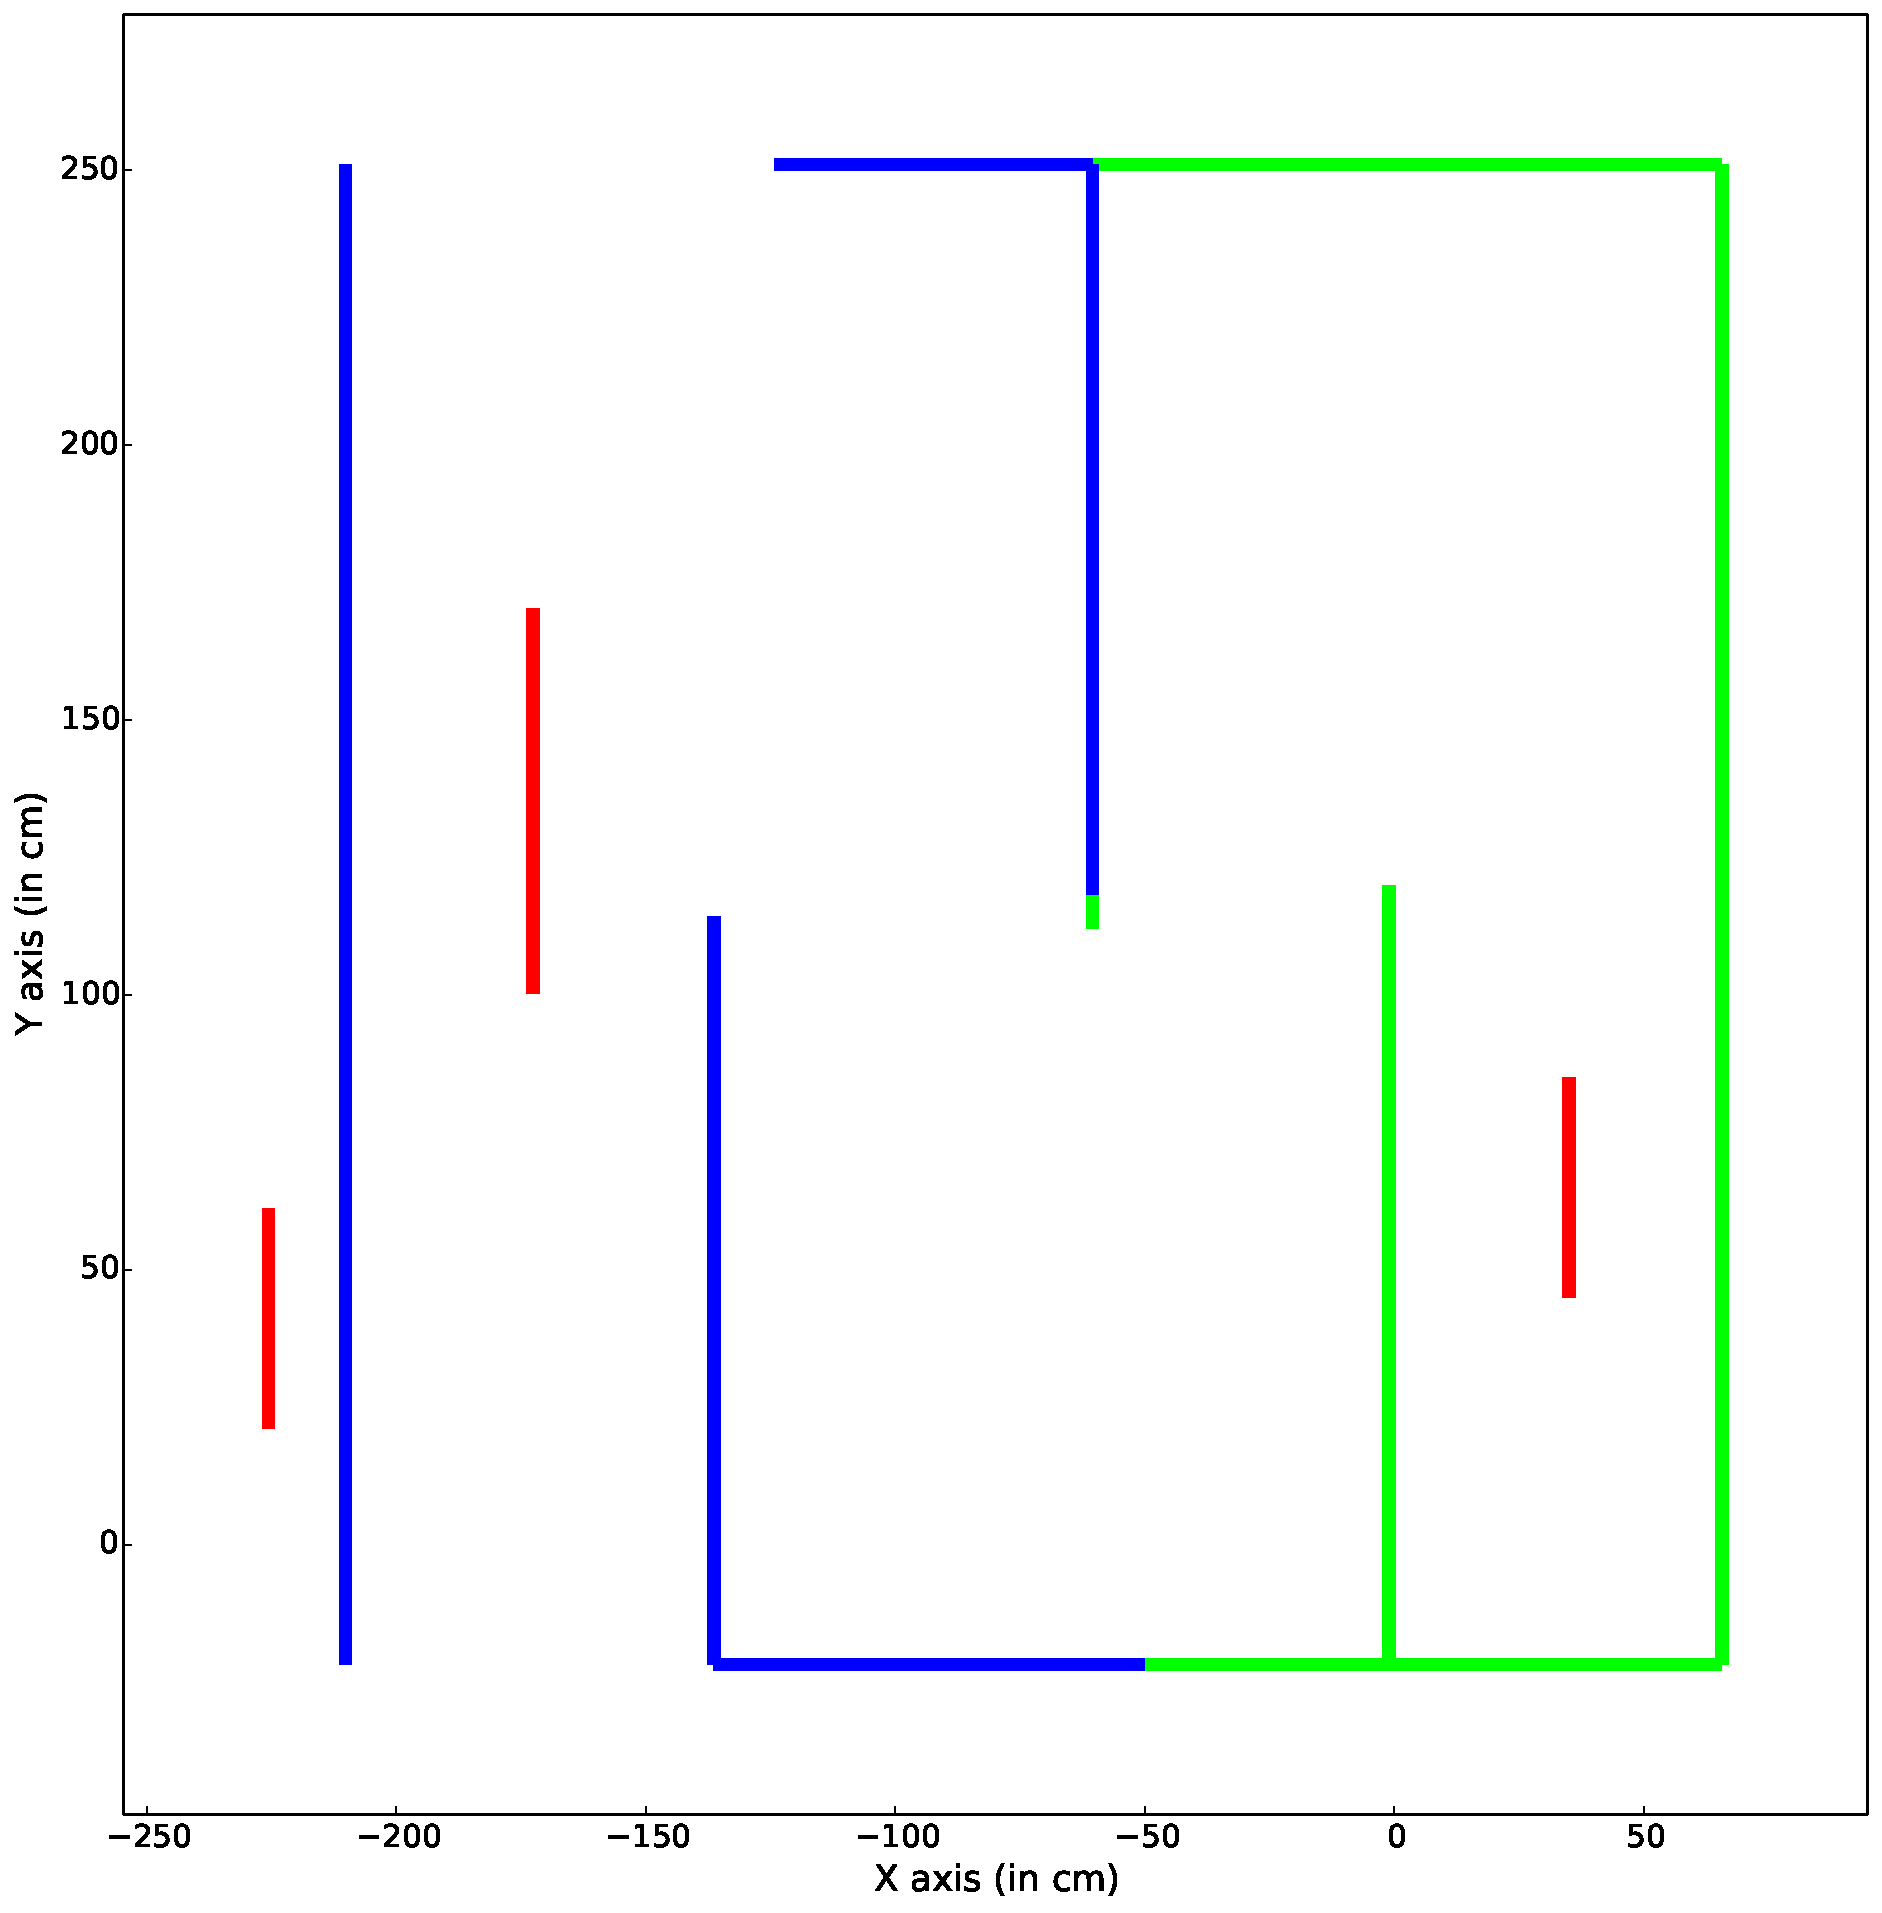
\includegraphics[scale=0.25]{./images/mmap4}
\caption[]{Merged maps from the two robots. Each local map is denoted either by red or green color and the red landmarks correspond to spurious landmarks. Note that the pose of vertical intersecting landmark are pinned together.}
\label{mmap4}
\end{figure}